\documentclass[conference]{IEEEtran}
\usepackage{cite}
\usepackage{amsmath,amssymb,amsfonts}
\newtheorem{definition}{Definition}
\newtheorem{theorem}{Theorem}
\usepackage{graphicx}
\usepackage{textcomp}
\usepackage{xcolor}
\usepackage[hidelinks]{hyperref}
%\usepackage{hyperref}
\usepackage{listings}
\usepackage{dblfloatfix} % Fix for float placement on pages
\usepackage{cuted} % inline full-width strips for side-by-side algorithm/description
%\usepackage{pbalance}
%%%
%---------
% Appendix figure (TikZ) --------------------
\usepackage{tikz}
\usetikzlibrary{arrows}
\usetikzlibrary{calc,arrows.meta,decorations.pathreplacing,shapes.geometric}
\usetikzlibrary{positioning,fit,backgrounds,shapes.symbols}
\usepackage{pgfplots}
\usepgfplotslibrary{groupplots}
\pgfplotsset{compat=1.16}

%\usepackage{tikz}
%\usetikzlibrary{arrows.meta,calc,angles,quotes}
% -------------------- Algorithms (boxed style, IEEE-friendly) --------------------
\usepackage[ruled,vlined]{algorithm2e}
\DontPrintSemicolon
\SetKwInput{KwIn}{Input}
\SetKwInput{KwOut}{Output}
\SetKw{KwTo}{to}
\SetKw{KwOr}{or}
%-----

% -------------------- Author notes --------------------
\newcommand{\todo}[1]{\textcolor{red}{\textbf{TODO}: {#1}}}

% Setup for listings style
\lstset{
    basicstyle=\ttfamily\footnotesize,
    breaklines=true,
    frame=tb,
    captionpos=b,
    backgroundcolor=\color{gray!5},
    commentstyle=\color{green!50!black},
    keywordstyle=\color{blue},
    stringstyle=\color{red},
    showstringspaces=false
}

\begin{document}
\setlength{\textfloatsep}{5pt plus 1pt minus 1pt}
\setlength{\floatsep}{4pt plus 1pt minus 1pt}
\setlength{\intextsep}{5pt plus 1pt minus 1pt}


\title{Bridging Natural Language to Verified Implementation: A Neuro-Symbolic High-Assurance MBSE Pipeline in SysML v2}

\author{
\IEEEauthorblockN{
Amer Tahat, David Hardin, Isaac Amundson, Junaid Babar,
Timothy A. Barclay, Janet Liu, Karl Hoech,\\ and Darren Cofer
}
\IEEEauthorblockA{
Collins Aerospace, an RTX Business\\
\{amer.tahat, david.hardin, isaac.amundson, junaid.babar,
timothy.a.barclay, janet.liu, karl.hoech,\\ darren.cofer\}@collins.com
}
}



\maketitle

\begin{abstract}
The development of high-confidence avionics systems demands rigorous allocation and end-to-end traceability from requirements to implementation, yet current Model-Based Systems Engineering (MBSE) environments provide little support for automated, mathematically verified allocation and traceability. While Generative AI (GenAI) offers a potential automation boon, its deployment in safety-critical workflows is severely constrained by hallucinations, prohibitive token costs, scarcity of open-source domain data, and restrictions on fine-tuning state-of-the-art proprietary models such as GPT-5.

To address these barriers, we introduce a neuro-symbolic \textbf{Spec--Code--Proof (SCP)} copilot that integrates Codex-class agents into the INSPECTA formal methods pipeline, developed on the DARPA PROVERS program. The pipeline translates natural-language requirements into \textbf{SysML v2} models containing formal \textbf{GUMBO} contracts, generates \textbf{HAMR} infrastructure code, and discharges \textbf{Logika} proofs, ensuring properties are mathematically preserved in the implementation. To enable specialization without fine-tuning, we introduce a \textit{Meta-Rule} learning methodology that functions as a verifiable surrogate for weight adaptation. Core to SCP is supervised self-healing and self-adaptation: successful in-context interactions are crystallized into persistent, expert-curated abstraction patterns, and Meta-Rules then drive a generate--verify--repair loop until the selected verification targets are satisfied within a given budget.

We evaluate our methodology on the Isolette infant-incubator system, a multi-subsystem HAMR/INSPECTA benchmark sourced from the FAA Requirements Engineering Management Handbook. Within the defined Isolette/HAMR target scope, our copilot achieved 100\% code-level verification and an 18$\times$ adjusted increase in development task throughput compared to a prompt-only baseline that, lacking Meta-Rules, failed to produce verifiable artifacts. This demonstrates a practical path to certification-facing automation under strict data and model governance constraints, while scoping the claim to HAMR-centric, toolchain-aware GUMBO repair; broader cross-system validation and additional rule books remain ongoing work.
\end{abstract}

\begin{IEEEkeywords}
SWE agents, Neuro-symbolic AI, Formal Methods, SysML v2, MBSE, Supervised Self-Healing, Supervised Meta-Rule Adaptation.
\end{IEEEkeywords}

DISTRIBUTION STATEMENT A. Approved for public distribution unlimited.


%====================================================================
\section{Introduction}

High-assurance avionics software development faces a persistent tension: system complexity continues to increase, while certification demands strong evidence that implementation faithfully realizes requirements and architectural intent. In practice, maintaining end-to-end traceability from natural-language requirements to architectural models to executable code remains costly and fragile. In many Model-Based Systems Engineering (MBSE) workflows, requirements allocation and refinement still involve manual, tool-fragmented steps that weaken (or sever) the link between model-level assurance and the software implementation correctness. The resulting drift is often detected late---during integration, verification/validation, or penetration testing---driving rework, schedule risk, and certification friction~\cite{hardin2025dasc}.

Large Language Models (LLMs) appear well-suited to assist with this decomposition by translating requirements into structured specifications, contracts, and implementation scaffolding~\cite{openai-gpt5-2-codex}. However, directly deploying LLMs in safety-critical workflows faces structural barriers. Beyond hallucinations and token-heavy prompting, aerospace environments face the \emph{fine-tuning bottleneck}: domain-representative data is often scarce or proprietary, and fine-tuning frontier proprietary models (e.g., GPT-5-class systems~\cite{bubeck2025earlyscienceaccelerationexperiments}) are typically restricted by vendor policy and/or cost~\cite{gpt5-system-card,openai-gpt5-2-codex}.

In this setting, the key challenge therefore is not merely to generate plausible formal text, but rather to produce a \emph{verified} artifact within bounded time, token, and human-review budgets. Recent theory on AI agents in verifiable settings provides a useful lens for this problem: past experience matters to the extent that it captures reusable algorithmic structure that reduces the time needed to solve new tasks~\cite{e28030332}. Viewed through this lens, the important quantity is not raw fluency alone, but \emph{cost per verified task}. This framing is particularly natural in MBSE pipelines where a formal checker is available and all candidate artifacts are filtered through hard acceptance gates.
%
%As a result, engineers are often left with unadapted general-purpose models or 
%As a result, engineers—particularly those without deep formal methods expertise—often resort to brittle, ad-hoc prompt engineering (or so-called `vibe coding'), which rarely produces the auditable evidence expected in certification-oriented development. 
These restrictions leave three highly desirable capabilities unmet:
(i) reducing token-heavy, brittle prompting; (ii) filtering or rejecting hallucinated behaviors with machine-checkable acceptance gates; and (iii) working from natural language specifications to produce reusable, auditable evidence that persists across runs.

To address these barriers, we introduce a neuro-symbolic \textbf{Spec--Code--Proof (SCP)} \emph{copilot}---a generate--verify--repair pipeline that turns natural-language requirements into traceable formal artifacts and verified implementations. SCP targets the three gaps above by (i) shifting effort from repeated token-heavy prompting into reusable intermediate artifacts; (ii) using formal verification as the primary acceptance gate to catch hallucinated or underspecified behavior; and (iii) providing a low-entry natural language interface while accumulating governed, version-controlled specialization knowledge. Our approach integrates Codex-class software engineering agents into the Industrial-Scale Proof Engineering for Critical Trustworthy Applications (\textbf{INSPECTA}) toolchain~\cite{hardin2025dasc}, developed on the DARPA Pipelined Reasoning of Verifiers Enabling Robust Systems (PROVERS) program. INSPECTA provides the formal backbone: \textbf{SysML v2}~\cite{sysmlv2_model_formalism_wg, sysmlv2_omg} captures the system architecture, \textbf{GUMBO}~\cite{gumbo, gumbo_galois} expresses behavioral assume/guarantee contracts, \textbf{HAMR}~\cite{hamr,HAMRsite} generates executable memory-safe infrastructure code, and \textbf{Logika}~\cite{HAMRsite} discharges proof obligations using SMT solvers (e.g., Z3~\cite{Z3} and CVC5~\cite{Barrett2011CVC4}). %The intended outcome is not merely synthesized code, but an auditable requirements-to-implementation workflow in which properties established at the model level are mechanically preserved in the generated code.
%--

This setting is challenging because a HAMR application is a layered assurance object, not a single text-to-code artifact. Requirements, SysML v2 architecture, GUMBO contracts, HAMR-generated Slang/Scala code, Logika/SMT obligations, build artifacts, diagnostics, and repair traces must remain mutually consistent; with seL4/Microkit targets, the model, generated implementation, platform glue, and proof-facing artifacts can span tens of thousands of lines across languages and verification layers~\cite{hamr,hamr-sel4,sel4_klein2009}. In a naive agentic workflow, upstream stochastic edits can trigger downstream failures and repeated replay of models, code, logs, and counterexamples. The research question is therefore how to combine stochastic generation with symbolic feedback so high-assurance AI assistance remains bounded, auditable, and repairable.

A major goal of INSPECTA is to create an auditable workflow where the toolchain mechanically preserves properties established at the model level in the generated code. However, while this infrastructure ensures correctness \emph{after} specification, the initial creation of formal models and contracts remains a manual, expertise-heavy exercise. Ideally, an agentic copilot would assist engineers in synthesizing these rigorous specifications from natural language directly; however, realizing this capability faces the critical barrier of effectively \emph{specializing} an LLM to such a complex, verification-centric toolchain under base-model fine-tuning restrictions.

Recent mechanistic interpretability results suggest that In-Context Learning (ICL) can act like an ``implicit fine-tuning'' process during inference~\cite{vonoswald2023transformers}, but the effect is transient: once the context window is cleared, the learned behavior is lost. In high-assurance settings, this ephemerality is a significant obstacle: it forces repeated token-heavy prompting and makes it difficult to govern, audit, or reuse what the model has ``learned'' across runs.

To stabilize this transient learning into a permanent asset, we introduce \textit{Meta-Rules}: persistent, human-readable formalization abstractions that \emph{crystallize} successful ICL interactions (derived from golden examples, tool feedback, and expert edits) into a reusable rule library. In the evaluated FSE rule book, a rule binds four kinds of reusable knowledge: linguistic triggers in requirements, semantic formalization choices, structural placement in SysML v2/GUMBO, and repair actions induced by HAMR/Slang/Logika feedback. Meta-Rules serve as a verifiable surrogate for black-box weight adaptation: instead of modifying parameters, the system externalizes adaptation into version-controlled artifacts that are (i) inspectable by humans, (ii) exercised by the toolchain, and (iii) constrained by formal verification.
%
In developer mode, the system iteratively proposes and refines Meta-Rules using semantic similarity metrics and INSPECTA tool (e.g., HAMR, Logika) feedback; only candidates that satisfy quantitative improvement criteria, pass verification, and receive human approval are retained. In user mode, the copilot injects this curated library into the context, effectively triggering the underlying implicit fine-tuning mechanism~\cite{vonoswald2023transformers} to behave as a domain-adapted agent. This allows us to bypass the aforementioned fine-tuning restrictions while achieving comparable specialization, driving a generate--verify--repair loop until model integration and code-level verification succeed.
%
In addition to consistently producing practical formally verifiable output at low cost (see Section~\ref{sec:evaluation}), and thus effectively lowering the entry barrier for users, this method systematically accumulates a dataset of verified repair trajectories, alleviating current data scarcity and paving the way for future fine-tuning as model accessibility improves.

By anchoring the development workflow in these governed, externalized artifacts rather than opaque model behaviors, our approach aligns with the industry's emerging \textit{Specification-Driven Development (SDD)} practices. Frameworks such as AWS Kiro~\cite{amazon2024mathematical} aim to curb ``vibe coding'' by structuring AI-assisted development around natural-language specifications and acceptance criteria rather than unconstrained prompt-driven generation. We extend this paradigm to \textit{Formal Specification-Driven Development (FSDD)} by making \emph{formal verification} the primary acceptance gate. In our workflow, specifications are refined into SysML v2 models and formal GUMBO contracts, then discharged through HAMR/Logika verification. This yields machine-checkable evidence alongside generated code, enabling a workflow aligned with certification demands for traceability, repeatability, as well as auditable assurance artifacts.

In summary, the main contributions of this paper are:
%--
\begin{enumerate}
    \item \textbf{Trustworthy English-to-Implementation Pipeline:} A multi-agent SCP generate--verify--repair loop workflow integrated with INSPECTA (SysML v2 + GUMBO + HAMR/Logika) that generates verified contracts and code from requirements.
    \item \textbf{Supervised Meta-Rules Self-Adaptation Algorithm:} A HAMR/INSPECTA-scoped adaptation method that externalizes successful in-context learning into persistent, verifier-gated Meta-Rules. Within the evaluated GUMBO--HAMR--Slang benchmark, semantic screening, HAMR/Logika feedback, and human approval guide a governed generate--verify--repair loop toward the defined verification targets.
    \item \textbf{System-Level HAMR Benchmark Evaluation:} An evaluation on the Isolette infant-incubator system~\cite{hatcliff2024isolette}, a realistic multi-subsystem HAMR/INSPECTA benchmark spanning requirements, SysML v2 models, GUMBO contracts, HAMR-generated Slang/Scala obligations, and Logika proof discharge. Within the scoped GUMBO FSE Rule book evaluation, Meta-Rules learned from a small solved file/subsystem example were reused on the remaining target files, converting a prompt-only failure into a fully verified target-scope run.
\end{enumerate}

The remainder of this paper is structured as follows. After establishing the SysML v2 GUMBO and HAMR/Logika background in Section~\ref{sec:gumbo}, Sections~\ref{sec:approach} and~\ref{sec:meta-learning} introduce the SCP architecture, the Meta-Rules framework, and the supervised self-adaptation algorithm. Section~\ref{sec:comparison} compares Meta-Rules to fine-tuning and transient prompting. Section~\ref{sec:example} then defines the Isolette/HAMR benchmark and reports the evaluation metrics and traces. Sections~\ref{sec:related-work}--\ref{sec:conclusion} discuss related work, limitations, and conclusions.

To foster community collaboration and accelerate future research, all toolchain source code, along with our curated dataset of successful repair trajectories, is released as open source~\cite{inspecta_repo}.%\footnote{URL to be added in the camera-ready version.%\url{https://github.com/loonwerks/INSPECTA-Spec-Code-Proof-Copilot}
%}

%As a result, engineers are often left with unadapted general-purpose models or brittle, ad-hoc prompt engineering, neither of which naturally produces the auditable evidence expected in certification-oriented development. This dilemma severely limits the utility of frontier models. 

%To address these barriers, we introduce a neuro-symbolic \textbf{Spec--Code--Proof (SCP)} pipeline that bridges natural-language requirements to verified implementation artifacts. Our approach integrates Codex-class software engineering agents into the DARPA PROVERS \textbf{INSPECTA} (Industrial-Scale Proof Engineering for Critical Trustworthy Applications) toolchain~\cite{hardin2025dasc}. INSPECTA provides the formal backbone: \textbf{SysML v2}~\cite{sysmlv2_model_formalism_wg, sysmlv2_omg} captures architecture, \textbf{GUMBO}~\cite{gumbo, gumbo_galois} expresses behavioral assume/guarantee contracts, \textbf{HAMR}~\cite{hamr,HAMRsite} generates executable memory-safe code, and \textbf{Logika}~\cite{HAMRsite} discharges proof obligations using SMT solvers (e.g., Z3~\cite{Z3} and CVC5~\cite{Barrett2011CVC4}). The intended outcome is not merely synthesized code, but an auditable requirements-to-implementation workflow in which properties established at the model level are mechanically preserved in the generated code.

%\subsection{Motivation: Adaptation Under Fine-Tuning Restrictions via Meta-Rules}
%A central technical challenge is how to adapt an LLM to this verification-centric toolchain under base-model fine-tuning restrictions. Recent mechanistic interpretability results suggest that In-Context Learning (ICL) can act like an ``implicit fine-tuning'' process during inference~\cite{vonoswald2023transformers}, but the effect is transient: once the context window is cleared, the learned behavior is lost. In high-assurance settings, this ephemerality is a practical obstacle: it forces repeated token-heavy prompting and makes it difficult to govern, audit, or reuse what the model ``learned'' across runs.

%We address this by introducing \textit{Meta-Rules}: persistent, human-readable formalization abstractions that \emph{crystallize} successful ICL interactions (derived from golden examples, tool feedback, and expert edits) into a reusable rule library. Meta-Rules serve as a verifiable surrogate for black-box weight adaptation: instead of modifying parameters, the system externalizes adaptation into version-controlled artifacts that are (i) inspectable by humans, (ii) exercised by the toolchain, and (iii) constrained by formal verification. In developer mode, the system iteratively proposes and refines Meta-Rules using semantic similarity metrics and HAMR/Logika feedback; only candidates that satisfy quantitative improvement criteria, pass verification, and receive human approval are retained. In user mode, the copilot can be triggered with a low entry-point prompt that applies the curated Meta-Rule library to drive a generate--verify--repair loop until model integration and code-level verification succeed.


%\subsection{Formal Specification-Driven Development (FSDD)}
%We align our work with the industry's emerging \textit{Specification-Driven Development (SDD)} practices. Frameworks such as GitHub Spec Kit~\cite{} and AWS Kiro~\cite{amazon2024mathematical} exemplify this trend by structuring AI-assisted coding around natural-language specifications, plans, and acceptance criteria, rather than unconstrained prompt-driven generation. These workflows aim to curb ``vibe coding'' by tracking the artifacts that guide implementation.

%We extend this paradigm to \textit{Formal Specification-Driven Development (FSDD)}. Our work complements emerging SDD workflows by making \emph{formal verification} the primary acceptance gate: specifications are refined into SysML v2 models and GUMBO contracts, then discharged through HAMR/Logika verification. This provides machine-checkable evidence alongside generated code, enabling a low-entry workflow that remains aligned with certification demands for traceability, repeatability, and auditable evidence.

%\subsection{Contributions and Organization}
%The main contributions of this paper are:
%\begin{enumerate}
   % \item \textbf{Trustworthy English-to-Implementation Pipeline:} A multi-agent SCP generate--verify--repair loop workflow integrated with INSPECTA (SysML v2 + GUMBO + HAMR/Logika) that generates verified contracts and code from requirements.
    %\item \textbf{Supervised Meta-Rules Adaptation:} A verifiable surrogate for fine-tuning that crystallizes ephemeral ICL behaviors into persistent Meta-Rules, enabling a governed generate--verify--repair loop driven by formal verification feedback and human approval.
    %\item \textbf{Empirical Evaluation:} An evaluation on the Isolette benchmark~\cite{hatcliff2024isolette} , demonstrating a substantial throughput increase and full verification success compared to a failing baseline.
%\end{enumerate}

%The remainder of this paper is organized as follows. Section~\ref{sec:gumbo} summarizes SysML v2 GUMBO contracts and the HAMR/Logika verification workflow. Section~\ref{sec:approach} presents the SCP neuro-symbolic architecture and the Meta-Rules methodology. Section~\ref{sec:comparison} compares Meta-Rules to fine-tuning and transient prompting, and discusses trade-offs. Section~\ref{sec:example} presents the Isolette running example. Section~\ref{sec:evaluation} details the experimental evaluation and metrics. Section~\ref{sec:related-work} discusses related work. Section~\ref{sec:limitations} discusses current limitations with future research directions, and Section~\ref{sec:conclusion} concludes.



\begin{figure*}[!t]
\centering
\resizebox{0.96\textwidth}{!}{% Merged agentic SCP + INSPECTA high-assurance development figure.
% Requires:
%   \usepackage{tikz}
%   \usetikzlibrary{arrows.meta,calc,positioning,fit,backgrounds,shapes.geometric}
% Recommended inclusion in an IEEE two-column paper:
%   \begin{figure*}[t]
%     \centering
%     \resizebox{0.96\textwidth}{!}{% Merged agentic SCP + INSPECTA high-assurance development figure.
% Requires:
%   \usepackage{tikz}
%   \usetikzlibrary{arrows.meta,calc,positioning,fit,backgrounds,shapes.geometric}
% Recommended inclusion in an IEEE two-column paper:
%   \begin{figure*}[t]
%     \centering
%     \resizebox{0.96\textwidth}{!}{% Merged agentic SCP + INSPECTA high-assurance development figure.
% Requires:
%   \usepackage{tikz}
%   \usetikzlibrary{arrows.meta,calc,positioning,fit,backgrounds,shapes.geometric}
% Recommended inclusion in an IEEE two-column paper:
%   \begin{figure*}[t]
%     \centering
%     \resizebox{0.96\textwidth}{!}{\input{figures/agentic_inspecta_toolchain_tikz}}
%     \caption{Agentic SCP/INSPECTA generate--verify--repair workflow.}
%     \label{fig:agentic-inspecta}
%   \end{figure*}

\begingroup
\definecolor{haLine}{RGB}{29,48,83}
\definecolor{haBlue}{RGB}{218,226,243}
\definecolor{haGreen}{RGB}{227,243,209}
\definecolor{haCream}{RGB}{241,238,235}
\definecolor{haProof}{RGB}{0,176,80}
\definecolor{haPurple}{RGB}{112,48,160}
\definecolor{agentBlue}{RGB}{221,235,247}
\definecolor{agentDark}{RGB}{31,78,121}
\definecolor{agentOrange}{RGB}{255,229,204}
\definecolor{agentRed}{RGB}{192,0,0}
\definecolor{agentYellow}{RGB}{255,242,204}

\tikzset{
  haBox/.style={draw=haLine, line width=0.58pt},
  haLayer/.style={haBox, fill=haBlue},
  haContract/.style={haBox, fill=haGreen},
  haCode/.style={haBox, fill=haCream},
  haWhite/.style={haBox, fill=white},
  haBinary/.style={draw=black, line width=0.58pt, fill=white},
  haPort/.style={haBox, fill=haBlue},
  haText/.style={font=\sffamily\fontsize{8.2}{8.9}\selectfont, inner sep=0pt, text=black},
  haBold/.style={font=\sffamily\bfseries\fontsize{8.2}{8.9}\selectfont, inner sep=0pt, text=black},
  haProofText/.style={font=\sffamily\fontsize{6.6}{7.0}\selectfont, inner sep=0pt, align=center, text=black},
  haMicro/.style={font=\sffamily\fontsize{4.5}{5}\selectfont, inner sep=0pt, text=black},
  haDataArrow/.style={-{Latex[length=5.8pt,width=5.8pt]}, draw=black, line width=1.35pt},
  haPurpleBoth/.style={{Latex[length=7.0pt,width=7.0pt]}-{Latex[length=7.0pt,width=7.0pt]}, draw=haPurple, line width=2.25pt},
  haProofArrow/.style={-{Triangle[length=9pt,width=8.5pt]}, draw=haProof, line width=3.35pt,
    dash pattern=on 4.1pt off 4.1pt, line cap=butt, line join=miter},
  haDot/.style={circle, fill=black, inner sep=0pt, minimum size=6.2pt},
  agentPanel/.style={draw=agentDark, rounded corners=3pt, line width=0.85pt, fill=agentBlue!45},
  agentBlock/.style={draw=agentDark, rounded corners=3pt, line width=0.75pt, fill=white},
  agentRules/.style={draw=agentDark, rounded corners=3pt, line width=0.75pt, fill=agentYellow},
  agentDiag/.style={draw=agentRed, rounded corners=3pt, line width=0.75pt, fill=red!7},
  agentTitle/.style={font=\sffamily\bfseries\fontsize{8.0}{8.6}\selectfont, inner sep=0pt, align=center, text=agentDark},
  agentText/.style={font=\sffamily\fontsize{6.6}{7.2}\selectfont, inner sep=0pt, align=center, text=black},
  agentTiny/.style={font=\sffamily\fontsize{5.8}{6.1}\selectfont, inner sep=1pt, align=center, text=black},
  specArrow/.style={-{Latex[length=6.8pt,width=6.2pt]}, draw=agentDark, line width=1.35pt},
  guideArrow/.style={-{Latex[length=5.5pt,width=5.0pt]}, draw=haProof!70!black, line width=1.0pt, dotted},
  repairArrow/.style={-{Latex[length=6.8pt,width=6.2pt]}, draw=haPurple, line width=1.35pt},
  failArrow/.style={-{Latex[length=6.8pt,width=6.2pt]}, draw=agentRed, line width=1.25pt, dashed},
  noteText/.style={font=\sffamily\fontsize{5.7}{6.1}\selectfont, inner sep=1pt, align=center, text=black}
}

\newcommand{\prooficon}[2]{%
  \begin{scope}[shift={(#1,#2)}]
    \draw[haBox, fill=white, rounded corners=1.4pt] (4,5) rectangle (22,22);
    \draw[haBox, fill=white, rounded corners=2.2pt] (0,0) rectangle (26,6);
    \draw[haBox, fill=white, rounded corners=2.0pt] (0,17) rectangle (10,22);
    \draw[haBox, fill=white] (13,13.8) circle (3.0);
    \draw[haBox, fill=white] (13,16.7) -- (9.6,22) -- (13,19.5) -- (16.4,22) -- cycle;
  \end{scope}}

\begin{tikzpicture}[x=1pt,y=-1pt]
  \path[use as bounding box] (-168,-4) rectangle (421,334);

  % ---------------- Agentic SCP panel ----------------
  \draw[agentPanel] (-166,0) rectangle (-12,318);
  \node[agentTitle] at (-89,12) {Agentic Spec-Code-Proof (SCP) Copilot};
  \node[agentTiny] at (-89,24) {bounded generate--verify--repair};

  \draw[agentBlock] (-153,35) rectangle (-25,60);
  \node[agentText] at (-89,47.5) {English Requirements\\architecture context};

  \draw[agentBlock] (-153,76) rectangle (-25,121);
  \node[agentText] at (-89,89) {Specification Agent};
  \node[agentTiny] at (-89,108) {propose / modify\\SysML v2 + GUMBO};

  \draw[agentRules] (-153,139) rectangle (-25,187);
  \node[agentText] at (-89,150) {Meta-Rules library};
  \node[agentTiny] at (-89,166) {verified patterns +\\semantic gates};
  \node[agentTiny] at (-89,180) {guide generation,\\bound retries};

  \draw[agentBlock] (-153,204) rectangle (-25,249);
  \node[agentText] at (-89,216) {Repair Agent};
  \node[agentTiny] at (-89,235) {suggested repair +\\modified plan};

  \draw[agentDiag] (-153,268) rectangle (-25,305);
  \node[agentText] at (-89,281) {Verifier Diagnostics};
  \node[agentTiny] at (-89,295) {error messages / counterexamples};

  \draw[specArrow] (-89,60) -- (-89,76);
  \draw[guideArrow] (-89,139) -- (-89,121);
  \draw[guideArrow] (-89,187) -- (-89,204);
  \draw[repairArrow] (-25,226) -- (-15,226) -- (-15,99) -- (-25,99);
  \node[agentTiny, fill=white, inner sep=1pt] at (-15,164) {retry plan};
  \draw[failArrow] (-89,268) -- (-89,249);
  \node[agentTiny, fill=white, inner sep=1pt] at (-132,257) {failure signal};

  % ---------------- Original high-assurance layer diagram ----------------

  \draw[haBinary] (0.00,288.47) rectangle (300.05,318.44);
  \draw[haWhite] (0.00,0.00) rectangle (300.05,75.48);
  \draw[haContract] (17.16,24.45) rectangle (116.54,65.64);
  \draw[haCode] (29.71,45.05) rectangle (105.82,65.64);
  \draw[haContract] (147.09,24.45) rectangle (246.47,65.64);
  \draw[haCode] (159.10,45.05) rectangle (235.21,65.64);
  \draw[haWhite] (0.00,137.62) rectangle (253.94,230.61);
  \draw[haContract] (261.46,137.62) rectangle (300.05,230.61);
  \draw[haLayer] (15.92,164.88) rectangle (104.61,220.01);
  \draw[haContract] (20.80,179.97) rectangle (101.79,220.01);
  \draw[haCode] (28.05,197.74) rectangle (98.31,220.04);
  \draw[haLayer] (153.11,164.85) rectangle (241.64,219.98);
  \draw[haContract] (157.99,179.95) rectangle (238.83,219.98);
  \draw[haCode] (165.24,197.72) rectangle (235.36,220.01);

  % Generated candidate specification arrows
\draw[specArrow] (-25,99) -- (-12,99) -- (-12,55) -- (16,55);
\draw[haPurpleBoth] (113.79,55.35) -- (151.14,55.35);
\draw[haPurpleBoth] (112.76,178.44) -- (145.47,178.44);
\draw[haDataArrow] (75.55,74.27) -- (75.55,146.27);
\draw[haDataArrow] (95.99,43.33) -- (95.99,188.79);
\draw[haDataArrow] (133.34,58.80) -- (133.34,161.76);
\draw[haDataArrow] (163.82,62.58) -- (163.82,172.38);
\draw[haDataArrow] (230.59,43.33) -- (230.59,207.38);
\draw[haDataArrow] (133.34,223.43) -- (133.34,296.51);
\draw[haDataArrow] (275.14,223.43) -- (275.14,296.51);



  \draw[haPort] (67.61,80.61) -- (82.98,80.61) -- (79.91,93.31) -- (70.68,93.31) -- cycle;
  \draw[haPort] (88.04,80.34) -- (103.42,80.34) -- (100.34,93.05) -- (91.12,93.05) -- cycle;
  \draw[haPort] (125.00,80.50) -- (140.38,80.50) -- (137.30,93.21) -- (128.08,93.21) -- cycle;
  \draw[haPort] (157.09,80.00) -- (172.46,80.00) -- (169.39,92.70) -- (160.16,92.70) -- cycle;
  \draw[haPort] (223.19,81.33) -- (238.56,81.33) -- (235.49,94.04) -- (226.26,94.04) -- cycle;
  \draw[haPort] (83.11,130.13) -- (67.73,130.13) -- (70.81,117.42) -- (80.04,117.42) -- cycle;
  \draw[haPort] (103.55,129.86) -- (88.17,129.86) -- (91.25,117.15) -- (100.47,117.15) -- cycle;
  \draw[haPort] (140.77,129.69) -- (125.39,129.69) -- (128.47,116.99) -- (137.69,116.99) -- cycle;
  \draw[haPort] (172.11,129.75) -- (156.73,129.75) -- (159.81,117.05) -- (169.03,117.05) -- cycle;
  \draw[haPort] (238.21,131.09) -- (222.83,131.09) -- (225.91,118.38) -- (235.13,118.38) -- cycle;
  \draw[haPort] (125.65,237.39) -- (141.03,237.39) -- (137.95,250.10) -- (128.73,250.10) -- cycle;
  \draw[haPort] (267.74,238.70) -- (283.11,238.70) -- (280.04,251.40) -- (270.81,251.40) -- cycle;
  \draw[haPort] (140.79,283.16) -- (125.41,283.16) -- (128.49,270.45) -- (137.71,270.45) -- cycle;
  \draw[haPort] (283.11,282.32) -- (267.74,282.32) -- (270.81,269.61) -- (280.04,269.61) -- cycle;

  \draw[haLayer] (0.00,90.23) rectangle (182.95,120.20);
  \draw[haLayer] (192.14,90.46) rectangle (300.05,120.43);
  \draw[haLayer] (0.00,245.70) rectangle (300.05,275.67);
  
 \draw[haProofArrow] (238.83,39.88) -- (362.41,39.88);
 \draw[haProofArrow] (283.11,99.70) -- (361.96,99.70);
 \draw[haProofArrow] (288.48,144.50) -- (361.11,144.50);
 \draw[haProofArrow] (235.21,190.73) -- (362.41,190.73);
 \draw[haProofArrow] (275.14,258.85) -- (362.41,258.85);

  % Generated candidate specification arrow endpoints
  \node[haDot] at (75.55,70.82) {};
  \node[haDot] at (95.99,39.88) {};
  \node[haDot] at (133.34,55.35) {};
  \node[haDot] at (163.82,59.13) {};
  \node[haDot] at (230.59,39.88) {};
  \node[haDot] at (133.34,219.98) {};
  \node[haDot] at (275.14,219.98) {};

  \prooficon{372.97}{28.79}
  \prooficon{372.52}{87.50}
  \prooficon{371.67}{132.31}
  \prooficon{372.97}{179.65}
  \prooficon{372.97}{247.76}

  % Verification-failure feedback bus.  Successful proof artifacts remain green.
  \draw[failArrow] (356,39.88) -- (340,39.88) -- (340,328) -- (-18,328) -- (-18,287) -- (-25,287);
  \node[haText, fill=white, text=agentRed] at (176,329) {Failure diagnostics returned to repair agent};
  \node[noteText, fill=white] at (305, 28) {Green dashed lines: proofs when Q.E.D.};

  % Labels.
  \node[haText,anchor=west] at (5.95,6.81) {System Architecture Model};
  \node[haText,anchor=west] at (23.11,31.01) {GUMBO Contract};
  \node[haText,anchor=west] at (47.42,55.41) {Component};
  \node[haText,anchor=west] at (153.04,31.01) {GUMBO Contract};
  \node[haText,anchor=west] at (176.81,55.41) {Component};
  \node[haBold,anchor=west] at (5.95,105.61) {HAMR};
  \node[haText,anchor=west] at (198.09,105.61) {Verified Synthesis};
  \node[haText,align=left,anchor=west] at (5.95,149.91) {Infrastructure\\Code (Slang/Scala)};
  \node[haText,align=left,anchor=west] at (267.41,149.91) {seL4};
  \node[haBold,anchor=west] at (5.95,260.61) {(Verified) Compiler};
  \node[haText,anchor=west] at (5.95,303.61) {Binary};
  \node[haText,anchor=west] at (31.11,171.81) {Component Stub};
  \node[haProofText] at (61.40,188.81) {Logika/Verus\\checkable contracts};
  \node[haText,align=center] at (63.18,207.50) {Rust/C/Slang};
  \node[haText,anchor=west] at (168.22,171.81) {Component Stub};
  \node[haProofText] at (198.40,188.81) {Logika/Verus\\checkable contracts};
  \node[haText,align=center] at (200.50,207.50) {Rust/C/Slang};
  \node[haText, anchor=south] at (132.70,173.91) {API};
%  \node[haMicro, anchor=north] at (132.70,179.41) {I};
  \node[haProofText] at (386.80,64.43) {Compositional\\Correctness\\Proofs};
  \node[haProofText] at (386.80,119.42) {Verified Code Gen\\Proofs};
  \node[haProofText] at (386.80,163.94) {Secure Kernel\\Proofs};
  \node[haProofText] at (386.80,214.64) {Component\\Correctness\\Proofs};
  \node[haProofText] at (386.80,281.72) {Correspondence\\Proofs};
\end{tikzpicture}
\endgroup
}
%     \caption{Agentic SCP/INSPECTA generate--verify--repair workflow.}
%     \label{fig:agentic-inspecta}
%   \end{figure*}

\begingroup
\definecolor{haLine}{RGB}{29,48,83}
\definecolor{haBlue}{RGB}{218,226,243}
\definecolor{haGreen}{RGB}{227,243,209}
\definecolor{haCream}{RGB}{241,238,235}
\definecolor{haProof}{RGB}{0,176,80}
\definecolor{haPurple}{RGB}{112,48,160}
\definecolor{agentBlue}{RGB}{221,235,247}
\definecolor{agentDark}{RGB}{31,78,121}
\definecolor{agentOrange}{RGB}{255,229,204}
\definecolor{agentRed}{RGB}{192,0,0}
\definecolor{agentYellow}{RGB}{255,242,204}

\tikzset{
  haBox/.style={draw=haLine, line width=0.58pt},
  haLayer/.style={haBox, fill=haBlue},
  haContract/.style={haBox, fill=haGreen},
  haCode/.style={haBox, fill=haCream},
  haWhite/.style={haBox, fill=white},
  haBinary/.style={draw=black, line width=0.58pt, fill=white},
  haPort/.style={haBox, fill=haBlue},
  haText/.style={font=\sffamily\fontsize{8.2}{8.9}\selectfont, inner sep=0pt, text=black},
  haBold/.style={font=\sffamily\bfseries\fontsize{8.2}{8.9}\selectfont, inner sep=0pt, text=black},
  haProofText/.style={font=\sffamily\fontsize{6.6}{7.0}\selectfont, inner sep=0pt, align=center, text=black},
  haMicro/.style={font=\sffamily\fontsize{4.5}{5}\selectfont, inner sep=0pt, text=black},
  haDataArrow/.style={-{Latex[length=5.8pt,width=5.8pt]}, draw=black, line width=1.35pt},
  haPurpleBoth/.style={{Latex[length=7.0pt,width=7.0pt]}-{Latex[length=7.0pt,width=7.0pt]}, draw=haPurple, line width=2.25pt},
  haProofArrow/.style={-{Triangle[length=9pt,width=8.5pt]}, draw=haProof, line width=3.35pt,
    dash pattern=on 4.1pt off 4.1pt, line cap=butt, line join=miter},
  haDot/.style={circle, fill=black, inner sep=0pt, minimum size=6.2pt},
  agentPanel/.style={draw=agentDark, rounded corners=3pt, line width=0.85pt, fill=agentBlue!45},
  agentBlock/.style={draw=agentDark, rounded corners=3pt, line width=0.75pt, fill=white},
  agentRules/.style={draw=agentDark, rounded corners=3pt, line width=0.75pt, fill=agentYellow},
  agentDiag/.style={draw=agentRed, rounded corners=3pt, line width=0.75pt, fill=red!7},
  agentTitle/.style={font=\sffamily\bfseries\fontsize{8.0}{8.6}\selectfont, inner sep=0pt, align=center, text=agentDark},
  agentText/.style={font=\sffamily\fontsize{6.6}{7.2}\selectfont, inner sep=0pt, align=center, text=black},
  agentTiny/.style={font=\sffamily\fontsize{5.8}{6.1}\selectfont, inner sep=1pt, align=center, text=black},
  specArrow/.style={-{Latex[length=6.8pt,width=6.2pt]}, draw=agentDark, line width=1.35pt},
  guideArrow/.style={-{Latex[length=5.5pt,width=5.0pt]}, draw=haProof!70!black, line width=1.0pt, dotted},
  repairArrow/.style={-{Latex[length=6.8pt,width=6.2pt]}, draw=haPurple, line width=1.35pt},
  failArrow/.style={-{Latex[length=6.8pt,width=6.2pt]}, draw=agentRed, line width=1.25pt, dashed},
  noteText/.style={font=\sffamily\fontsize{5.7}{6.1}\selectfont, inner sep=1pt, align=center, text=black}
}

\newcommand{\prooficon}[2]{%
  \begin{scope}[shift={(#1,#2)}]
    \draw[haBox, fill=white, rounded corners=1.4pt] (4,5) rectangle (22,22);
    \draw[haBox, fill=white, rounded corners=2.2pt] (0,0) rectangle (26,6);
    \draw[haBox, fill=white, rounded corners=2.0pt] (0,17) rectangle (10,22);
    \draw[haBox, fill=white] (13,13.8) circle (3.0);
    \draw[haBox, fill=white] (13,16.7) -- (9.6,22) -- (13,19.5) -- (16.4,22) -- cycle;
  \end{scope}}

\begin{tikzpicture}[x=1pt,y=-1pt]
  \path[use as bounding box] (-168,-4) rectangle (421,334);

  % ---------------- Agentic SCP panel ----------------
  \draw[agentPanel] (-166,0) rectangle (-12,318);
  \node[agentTitle] at (-89,12) {Agentic Spec-Code-Proof (SCP) Copilot};
  \node[agentTiny] at (-89,24) {bounded generate--verify--repair};

  \draw[agentBlock] (-153,35) rectangle (-25,60);
  \node[agentText] at (-89,47.5) {English Requirements\\architecture context};

  \draw[agentBlock] (-153,76) rectangle (-25,121);
  \node[agentText] at (-89,89) {Specification Agent};
  \node[agentTiny] at (-89,108) {propose / modify\\SysML v2 + GUMBO};

  \draw[agentRules] (-153,139) rectangle (-25,187);
  \node[agentText] at (-89,150) {Meta-Rules library};
  \node[agentTiny] at (-89,166) {verified patterns +\\semantic gates};
  \node[agentTiny] at (-89,180) {guide generation,\\bound retries};

  \draw[agentBlock] (-153,204) rectangle (-25,249);
  \node[agentText] at (-89,216) {Repair Agent};
  \node[agentTiny] at (-89,235) {suggested repair +\\modified plan};

  \draw[agentDiag] (-153,268) rectangle (-25,305);
  \node[agentText] at (-89,281) {Verifier Diagnostics};
  \node[agentTiny] at (-89,295) {error messages / counterexamples};

  \draw[specArrow] (-89,60) -- (-89,76);
  \draw[guideArrow] (-89,139) -- (-89,121);
  \draw[guideArrow] (-89,187) -- (-89,204);
  \draw[repairArrow] (-25,226) -- (-15,226) -- (-15,99) -- (-25,99);
  \node[agentTiny, fill=white, inner sep=1pt] at (-15,164) {retry plan};
  \draw[failArrow] (-89,268) -- (-89,249);
  \node[agentTiny, fill=white, inner sep=1pt] at (-132,257) {failure signal};

  % ---------------- Original high-assurance layer diagram ----------------

  \draw[haBinary] (0.00,288.47) rectangle (300.05,318.44);
  \draw[haWhite] (0.00,0.00) rectangle (300.05,75.48);
  \draw[haContract] (17.16,24.45) rectangle (116.54,65.64);
  \draw[haCode] (29.71,45.05) rectangle (105.82,65.64);
  \draw[haContract] (147.09,24.45) rectangle (246.47,65.64);
  \draw[haCode] (159.10,45.05) rectangle (235.21,65.64);
  \draw[haWhite] (0.00,137.62) rectangle (253.94,230.61);
  \draw[haContract] (261.46,137.62) rectangle (300.05,230.61);
  \draw[haLayer] (15.92,164.88) rectangle (104.61,220.01);
  \draw[haContract] (20.80,179.97) rectangle (101.79,220.01);
  \draw[haCode] (28.05,197.74) rectangle (98.31,220.04);
  \draw[haLayer] (153.11,164.85) rectangle (241.64,219.98);
  \draw[haContract] (157.99,179.95) rectangle (238.83,219.98);
  \draw[haCode] (165.24,197.72) rectangle (235.36,220.01);

  % Generated candidate specification arrows
\draw[specArrow] (-25,99) -- (-12,99) -- (-12,55) -- (16,55);
\draw[haPurpleBoth] (113.79,55.35) -- (151.14,55.35);
\draw[haPurpleBoth] (112.76,178.44) -- (145.47,178.44);
\draw[haDataArrow] (75.55,74.27) -- (75.55,146.27);
\draw[haDataArrow] (95.99,43.33) -- (95.99,188.79);
\draw[haDataArrow] (133.34,58.80) -- (133.34,161.76);
\draw[haDataArrow] (163.82,62.58) -- (163.82,172.38);
\draw[haDataArrow] (230.59,43.33) -- (230.59,207.38);
\draw[haDataArrow] (133.34,223.43) -- (133.34,296.51);
\draw[haDataArrow] (275.14,223.43) -- (275.14,296.51);



  \draw[haPort] (67.61,80.61) -- (82.98,80.61) -- (79.91,93.31) -- (70.68,93.31) -- cycle;
  \draw[haPort] (88.04,80.34) -- (103.42,80.34) -- (100.34,93.05) -- (91.12,93.05) -- cycle;
  \draw[haPort] (125.00,80.50) -- (140.38,80.50) -- (137.30,93.21) -- (128.08,93.21) -- cycle;
  \draw[haPort] (157.09,80.00) -- (172.46,80.00) -- (169.39,92.70) -- (160.16,92.70) -- cycle;
  \draw[haPort] (223.19,81.33) -- (238.56,81.33) -- (235.49,94.04) -- (226.26,94.04) -- cycle;
  \draw[haPort] (83.11,130.13) -- (67.73,130.13) -- (70.81,117.42) -- (80.04,117.42) -- cycle;
  \draw[haPort] (103.55,129.86) -- (88.17,129.86) -- (91.25,117.15) -- (100.47,117.15) -- cycle;
  \draw[haPort] (140.77,129.69) -- (125.39,129.69) -- (128.47,116.99) -- (137.69,116.99) -- cycle;
  \draw[haPort] (172.11,129.75) -- (156.73,129.75) -- (159.81,117.05) -- (169.03,117.05) -- cycle;
  \draw[haPort] (238.21,131.09) -- (222.83,131.09) -- (225.91,118.38) -- (235.13,118.38) -- cycle;
  \draw[haPort] (125.65,237.39) -- (141.03,237.39) -- (137.95,250.10) -- (128.73,250.10) -- cycle;
  \draw[haPort] (267.74,238.70) -- (283.11,238.70) -- (280.04,251.40) -- (270.81,251.40) -- cycle;
  \draw[haPort] (140.79,283.16) -- (125.41,283.16) -- (128.49,270.45) -- (137.71,270.45) -- cycle;
  \draw[haPort] (283.11,282.32) -- (267.74,282.32) -- (270.81,269.61) -- (280.04,269.61) -- cycle;

  \draw[haLayer] (0.00,90.23) rectangle (182.95,120.20);
  \draw[haLayer] (192.14,90.46) rectangle (300.05,120.43);
  \draw[haLayer] (0.00,245.70) rectangle (300.05,275.67);
  
 \draw[haProofArrow] (238.83,39.88) -- (362.41,39.88);
 \draw[haProofArrow] (283.11,99.70) -- (361.96,99.70);
 \draw[haProofArrow] (288.48,144.50) -- (361.11,144.50);
 \draw[haProofArrow] (235.21,190.73) -- (362.41,190.73);
 \draw[haProofArrow] (275.14,258.85) -- (362.41,258.85);

  % Generated candidate specification arrow endpoints
  \node[haDot] at (75.55,70.82) {};
  \node[haDot] at (95.99,39.88) {};
  \node[haDot] at (133.34,55.35) {};
  \node[haDot] at (163.82,59.13) {};
  \node[haDot] at (230.59,39.88) {};
  \node[haDot] at (133.34,219.98) {};
  \node[haDot] at (275.14,219.98) {};

  \prooficon{372.97}{28.79}
  \prooficon{372.52}{87.50}
  \prooficon{371.67}{132.31}
  \prooficon{372.97}{179.65}
  \prooficon{372.97}{247.76}

  % Verification-failure feedback bus.  Successful proof artifacts remain green.
  \draw[failArrow] (356,39.88) -- (340,39.88) -- (340,328) -- (-18,328) -- (-18,287) -- (-25,287);
  \node[haText, fill=white, text=agentRed] at (176,329) {Failure diagnostics returned to repair agent};
  \node[noteText, fill=white] at (305, 28) {Green dashed lines: proofs when Q.E.D.};

  % Labels.
  \node[haText,anchor=west] at (5.95,6.81) {System Architecture Model};
  \node[haText,anchor=west] at (23.11,31.01) {GUMBO Contract};
  \node[haText,anchor=west] at (47.42,55.41) {Component};
  \node[haText,anchor=west] at (153.04,31.01) {GUMBO Contract};
  \node[haText,anchor=west] at (176.81,55.41) {Component};
  \node[haBold,anchor=west] at (5.95,105.61) {HAMR};
  \node[haText,anchor=west] at (198.09,105.61) {Verified Synthesis};
  \node[haText,align=left,anchor=west] at (5.95,149.91) {Infrastructure\\Code (Slang/Scala)};
  \node[haText,align=left,anchor=west] at (267.41,149.91) {seL4};
  \node[haBold,anchor=west] at (5.95,260.61) {(Verified) Compiler};
  \node[haText,anchor=west] at (5.95,303.61) {Binary};
  \node[haText,anchor=west] at (31.11,171.81) {Component Stub};
  \node[haProofText] at (61.40,188.81) {Logika/Verus\\checkable contracts};
  \node[haText,align=center] at (63.18,207.50) {Rust/C/Slang};
  \node[haText,anchor=west] at (168.22,171.81) {Component Stub};
  \node[haProofText] at (198.40,188.81) {Logika/Verus\\checkable contracts};
  \node[haText,align=center] at (200.50,207.50) {Rust/C/Slang};
  \node[haText, anchor=south] at (132.70,173.91) {API};
%  \node[haMicro, anchor=north] at (132.70,179.41) {I};
  \node[haProofText] at (386.80,64.43) {Compositional\\Correctness\\Proofs};
  \node[haProofText] at (386.80,119.42) {Verified Code Gen\\Proofs};
  \node[haProofText] at (386.80,163.94) {Secure Kernel\\Proofs};
  \node[haProofText] at (386.80,214.64) {Component\\Correctness\\Proofs};
  \node[haProofText] at (386.80,281.72) {Correspondence\\Proofs};
\end{tikzpicture}
\endgroup
}
%     \caption{Agentic SCP/INSPECTA generate--verify--repair workflow.}
%     \label{fig:agentic-inspecta}
%   \end{figure*}

\begingroup
\definecolor{haLine}{RGB}{29,48,83}
\definecolor{haBlue}{RGB}{218,226,243}
\definecolor{haGreen}{RGB}{227,243,209}
\definecolor{haCream}{RGB}{241,238,235}
\definecolor{haProof}{RGB}{0,176,80}
\definecolor{haPurple}{RGB}{112,48,160}
\definecolor{agentBlue}{RGB}{221,235,247}
\definecolor{agentDark}{RGB}{31,78,121}
\definecolor{agentOrange}{RGB}{255,229,204}
\definecolor{agentRed}{RGB}{192,0,0}
\definecolor{agentYellow}{RGB}{255,242,204}

\tikzset{
  haBox/.style={draw=haLine, line width=0.58pt},
  haLayer/.style={haBox, fill=haBlue},
  haContract/.style={haBox, fill=haGreen},
  haCode/.style={haBox, fill=haCream},
  haWhite/.style={haBox, fill=white},
  haBinary/.style={draw=black, line width=0.58pt, fill=white},
  haPort/.style={haBox, fill=haBlue},
  haText/.style={font=\sffamily\fontsize{8.2}{8.9}\selectfont, inner sep=0pt, text=black},
  haBold/.style={font=\sffamily\bfseries\fontsize{8.2}{8.9}\selectfont, inner sep=0pt, text=black},
  haProofText/.style={font=\sffamily\fontsize{6.6}{7.0}\selectfont, inner sep=0pt, align=center, text=black},
  haMicro/.style={font=\sffamily\fontsize{4.5}{5}\selectfont, inner sep=0pt, text=black},
  haDataArrow/.style={-{Latex[length=5.8pt,width=5.8pt]}, draw=black, line width=1.35pt},
  haPurpleBoth/.style={{Latex[length=7.0pt,width=7.0pt]}-{Latex[length=7.0pt,width=7.0pt]}, draw=haPurple, line width=2.25pt},
  haProofArrow/.style={-{Triangle[length=9pt,width=8.5pt]}, draw=haProof, line width=3.35pt,
    dash pattern=on 4.1pt off 4.1pt, line cap=butt, line join=miter},
  haDot/.style={circle, fill=black, inner sep=0pt, minimum size=6.2pt},
  agentPanel/.style={draw=agentDark, rounded corners=3pt, line width=0.85pt, fill=agentBlue!45},
  agentBlock/.style={draw=agentDark, rounded corners=3pt, line width=0.75pt, fill=white},
  agentRules/.style={draw=agentDark, rounded corners=3pt, line width=0.75pt, fill=agentYellow},
  agentDiag/.style={draw=agentRed, rounded corners=3pt, line width=0.75pt, fill=red!7},
  agentTitle/.style={font=\sffamily\bfseries\fontsize{8.0}{8.6}\selectfont, inner sep=0pt, align=center, text=agentDark},
  agentText/.style={font=\sffamily\fontsize{6.6}{7.2}\selectfont, inner sep=0pt, align=center, text=black},
  agentTiny/.style={font=\sffamily\fontsize{5.8}{6.1}\selectfont, inner sep=1pt, align=center, text=black},
  specArrow/.style={-{Latex[length=6.8pt,width=6.2pt]}, draw=agentDark, line width=1.35pt},
  guideArrow/.style={-{Latex[length=5.5pt,width=5.0pt]}, draw=haProof!70!black, line width=1.0pt, dotted},
  repairArrow/.style={-{Latex[length=6.8pt,width=6.2pt]}, draw=haPurple, line width=1.35pt},
  failArrow/.style={-{Latex[length=6.8pt,width=6.2pt]}, draw=agentRed, line width=1.25pt, dashed},
  noteText/.style={font=\sffamily\fontsize{5.7}{6.1}\selectfont, inner sep=1pt, align=center, text=black}
}

\newcommand{\prooficon}[2]{%
  \begin{scope}[shift={(#1,#2)}]
    \draw[haBox, fill=white, rounded corners=1.4pt] (4,5) rectangle (22,22);
    \draw[haBox, fill=white, rounded corners=2.2pt] (0,0) rectangle (26,6);
    \draw[haBox, fill=white, rounded corners=2.0pt] (0,17) rectangle (10,22);
    \draw[haBox, fill=white] (13,13.8) circle (3.0);
    \draw[haBox, fill=white] (13,16.7) -- (9.6,22) -- (13,19.5) -- (16.4,22) -- cycle;
  \end{scope}}

\begin{tikzpicture}[x=1pt,y=-1pt]
  \path[use as bounding box] (-168,-4) rectangle (421,334);

  % ---------------- Agentic SCP panel ----------------
  \draw[agentPanel] (-166,0) rectangle (-12,318);
  \node[agentTitle] at (-89,12) {Agentic Spec-Code-Proof (SCP) Copilot};
  \node[agentTiny] at (-89,24) {bounded generate--verify--repair};

  \draw[agentBlock] (-153,35) rectangle (-25,60);
  \node[agentText] at (-89,47.5) {English Requirements\\architecture context};

  \draw[agentBlock] (-153,76) rectangle (-25,121);
  \node[agentText] at (-89,89) {Specification Agent};
  \node[agentTiny] at (-89,108) {propose / modify\\SysML v2 + GUMBO};

  \draw[agentRules] (-153,139) rectangle (-25,187);
  \node[agentText] at (-89,150) {Meta-Rules library};
  \node[agentTiny] at (-89,166) {verified patterns +\\semantic gates};
  \node[agentTiny] at (-89,180) {guide generation,\\bound retries};

  \draw[agentBlock] (-153,204) rectangle (-25,249);
  \node[agentText] at (-89,216) {Repair Agent};
  \node[agentTiny] at (-89,235) {suggested repair +\\modified plan};

  \draw[agentDiag] (-153,268) rectangle (-25,305);
  \node[agentText] at (-89,281) {Verifier Diagnostics};
  \node[agentTiny] at (-89,295) {error messages / counterexamples};

  \draw[specArrow] (-89,60) -- (-89,76);
  \draw[guideArrow] (-89,139) -- (-89,121);
  \draw[guideArrow] (-89,187) -- (-89,204);
  \draw[repairArrow] (-25,226) -- (-15,226) -- (-15,99) -- (-25,99);
  \node[agentTiny, fill=white, inner sep=1pt] at (-15,164) {retry plan};
  \draw[failArrow] (-89,268) -- (-89,249);
  \node[agentTiny, fill=white, inner sep=1pt] at (-132,257) {failure signal};

  % ---------------- Original high-assurance layer diagram ----------------

  \draw[haBinary] (0.00,288.47) rectangle (300.05,318.44);
  \draw[haWhite] (0.00,0.00) rectangle (300.05,75.48);
  \draw[haContract] (17.16,24.45) rectangle (116.54,65.64);
  \draw[haCode] (29.71,45.05) rectangle (105.82,65.64);
  \draw[haContract] (147.09,24.45) rectangle (246.47,65.64);
  \draw[haCode] (159.10,45.05) rectangle (235.21,65.64);
  \draw[haWhite] (0.00,137.62) rectangle (253.94,230.61);
  \draw[haContract] (261.46,137.62) rectangle (300.05,230.61);
  \draw[haLayer] (15.92,164.88) rectangle (104.61,220.01);
  \draw[haContract] (20.80,179.97) rectangle (101.79,220.01);
  \draw[haCode] (28.05,197.74) rectangle (98.31,220.04);
  \draw[haLayer] (153.11,164.85) rectangle (241.64,219.98);
  \draw[haContract] (157.99,179.95) rectangle (238.83,219.98);
  \draw[haCode] (165.24,197.72) rectangle (235.36,220.01);

  % Generated candidate specification arrows
\draw[specArrow] (-25,99) -- (-12,99) -- (-12,55) -- (16,55);
\draw[haPurpleBoth] (113.79,55.35) -- (151.14,55.35);
\draw[haPurpleBoth] (112.76,178.44) -- (145.47,178.44);
\draw[haDataArrow] (75.55,74.27) -- (75.55,146.27);
\draw[haDataArrow] (95.99,43.33) -- (95.99,188.79);
\draw[haDataArrow] (133.34,58.80) -- (133.34,161.76);
\draw[haDataArrow] (163.82,62.58) -- (163.82,172.38);
\draw[haDataArrow] (230.59,43.33) -- (230.59,207.38);
\draw[haDataArrow] (133.34,223.43) -- (133.34,296.51);
\draw[haDataArrow] (275.14,223.43) -- (275.14,296.51);



  \draw[haPort] (67.61,80.61) -- (82.98,80.61) -- (79.91,93.31) -- (70.68,93.31) -- cycle;
  \draw[haPort] (88.04,80.34) -- (103.42,80.34) -- (100.34,93.05) -- (91.12,93.05) -- cycle;
  \draw[haPort] (125.00,80.50) -- (140.38,80.50) -- (137.30,93.21) -- (128.08,93.21) -- cycle;
  \draw[haPort] (157.09,80.00) -- (172.46,80.00) -- (169.39,92.70) -- (160.16,92.70) -- cycle;
  \draw[haPort] (223.19,81.33) -- (238.56,81.33) -- (235.49,94.04) -- (226.26,94.04) -- cycle;
  \draw[haPort] (83.11,130.13) -- (67.73,130.13) -- (70.81,117.42) -- (80.04,117.42) -- cycle;
  \draw[haPort] (103.55,129.86) -- (88.17,129.86) -- (91.25,117.15) -- (100.47,117.15) -- cycle;
  \draw[haPort] (140.77,129.69) -- (125.39,129.69) -- (128.47,116.99) -- (137.69,116.99) -- cycle;
  \draw[haPort] (172.11,129.75) -- (156.73,129.75) -- (159.81,117.05) -- (169.03,117.05) -- cycle;
  \draw[haPort] (238.21,131.09) -- (222.83,131.09) -- (225.91,118.38) -- (235.13,118.38) -- cycle;
  \draw[haPort] (125.65,237.39) -- (141.03,237.39) -- (137.95,250.10) -- (128.73,250.10) -- cycle;
  \draw[haPort] (267.74,238.70) -- (283.11,238.70) -- (280.04,251.40) -- (270.81,251.40) -- cycle;
  \draw[haPort] (140.79,283.16) -- (125.41,283.16) -- (128.49,270.45) -- (137.71,270.45) -- cycle;
  \draw[haPort] (283.11,282.32) -- (267.74,282.32) -- (270.81,269.61) -- (280.04,269.61) -- cycle;

  \draw[haLayer] (0.00,90.23) rectangle (182.95,120.20);
  \draw[haLayer] (192.14,90.46) rectangle (300.05,120.43);
  \draw[haLayer] (0.00,245.70) rectangle (300.05,275.67);
  
 \draw[haProofArrow] (238.83,39.88) -- (362.41,39.88);
 \draw[haProofArrow] (283.11,99.70) -- (361.96,99.70);
 \draw[haProofArrow] (288.48,144.50) -- (361.11,144.50);
 \draw[haProofArrow] (235.21,190.73) -- (362.41,190.73);
 \draw[haProofArrow] (275.14,258.85) -- (362.41,258.85);

  % Generated candidate specification arrow endpoints
  \node[haDot] at (75.55,70.82) {};
  \node[haDot] at (95.99,39.88) {};
  \node[haDot] at (133.34,55.35) {};
  \node[haDot] at (163.82,59.13) {};
  \node[haDot] at (230.59,39.88) {};
  \node[haDot] at (133.34,219.98) {};
  \node[haDot] at (275.14,219.98) {};

  \prooficon{372.97}{28.79}
  \prooficon{372.52}{87.50}
  \prooficon{371.67}{132.31}
  \prooficon{372.97}{179.65}
  \prooficon{372.97}{247.76}

  % Verification-failure feedback bus.  Successful proof artifacts remain green.
  \draw[failArrow] (356,39.88) -- (340,39.88) -- (340,328) -- (-18,328) -- (-18,287) -- (-25,287);
  \node[haText, fill=white, text=agentRed] at (176,329) {Failure diagnostics returned to repair agent};
  \node[noteText, fill=white] at (305, 28) {Green dashed lines: proofs when Q.E.D.};

  % Labels.
  \node[haText,anchor=west] at (5.95,6.81) {System Architecture Model};
  \node[haText,anchor=west] at (23.11,31.01) {GUMBO Contract};
  \node[haText,anchor=west] at (47.42,55.41) {Component};
  \node[haText,anchor=west] at (153.04,31.01) {GUMBO Contract};
  \node[haText,anchor=west] at (176.81,55.41) {Component};
  \node[haBold,anchor=west] at (5.95,105.61) {HAMR};
  \node[haText,anchor=west] at (198.09,105.61) {Verified Synthesis};
  \node[haText,align=left,anchor=west] at (5.95,149.91) {Infrastructure\\Code (Slang/Scala)};
  \node[haText,align=left,anchor=west] at (267.41,149.91) {seL4};
  \node[haBold,anchor=west] at (5.95,260.61) {(Verified) Compiler};
  \node[haText,anchor=west] at (5.95,303.61) {Binary};
  \node[haText,anchor=west] at (31.11,171.81) {Component Stub};
  \node[haProofText] at (61.40,188.81) {Logika/Verus\\checkable contracts};
  \node[haText,align=center] at (63.18,207.50) {Rust/C/Slang};
  \node[haText,anchor=west] at (168.22,171.81) {Component Stub};
  \node[haProofText] at (198.40,188.81) {Logika/Verus\\checkable contracts};
  \node[haText,align=center] at (200.50,207.50) {Rust/C/Slang};
  \node[haText, anchor=south] at (132.70,173.91) {API};
%  \node[haMicro, anchor=north] at (132.70,179.41) {I};
  \node[haProofText] at (386.80,64.43) {Compositional\\Correctness\\Proofs};
  \node[haProofText] at (386.80,119.42) {Verified Code Gen\\Proofs};
  \node[haProofText] at (386.80,163.94) {Secure Kernel\\Proofs};
  \node[haProofText] at (386.80,214.64) {Component\\Correctness\\Proofs};
  \node[haProofText] at (386.80,281.72) {Correspondence\\Proofs};
\end{tikzpicture}
\endgroup
}
\caption{Agentic SCP/INSPECTA workflow integrating the high-assurance development layers with a Meta-Rule-guided generate--verify--repair loop. Green dashed arrows denote successful proof artifacts; the red dashed arrow denotes verifier-failure diagnostics returned to the repair agent for a bounded retry.}
\label{fig:agentic-inspecta}
\vspace{-0.4em}
\end{figure*}

%====================================================================
\section{Background}
\label{sec:background}

\subsection{INSPECTA High-Assurance System Development and Verification}
\label{sec:gumbo}

The development of safety-critical systems, including digital avionics systems, requires rigorous evidence that implementations faithfully realize their requirements. The DARPA PROVERS INSPECTA toolchain provides this verifiable setting by automatically integrating architectural design, code generation, and formal verification capabilities. Specifically, 
\begin{itemize}
\item SysML v2 and GUMBO: Architecture models are captured in SysML v2, which natively supports a textual representation amenable to LLM processing. These models are annotated with GUMBO contracts. GUMBO allows engineers to attach formal specifications in the form of \textit{assumptions} and \textit{guarantees} directly to components (parts) in the architecture model.

\item HAMR and Logika: The HAMR framework analyzes these models to generate memory-safe executable infrastructure code in languages like Slang/Scala (default and target of this paper), C, or Rust; mapping GUMBO assumptions and guarantees to formal verifiable \textit{requires} and \textit{ensures} clauses, respectively. Subsequently, in the case of Scala/Slang, the Logika formal verification framework uses SMT solvers (e.g., Z3, CVC5) to discharge proof obligations, ensuring the component application code (developed manually or via LLM assistance) satisfies its GUMBO contracts across the entire state space.

\item Finally, Rust and Verus: For Rust targets, HAMR generates Verus verification annotations. Verus allows developers to specify and prove properties using Rust’s ownership model, mapping GUMBO assumptions and guarantees to Verus \textit{requires} and \textit{ensures} blocks, respectively. In this paper, our SCP copilot supports the default behavior. 
\end{itemize}

Figure~\ref{fig:agentic-inspecta} merges the INSPECTA assurance stack with the SCP agentic repair loop used in this paper. The specification agent proposes or updates SysML v2/GUMBO contracts under guidance from persistent Meta-Rules. The verifier stack then acts as a hard gate: successful checks emit proof artifacts, while failed checks return diagnostics and counterexamples to the repair agent. The repair agent converts those diagnostics into a suggested repair and modified plan, which is fed back to the specification agent for a bounded retry. In this sense, Meta-Rules and verifiers act together as guided generation: they constrain the search space before expensive multilayer verification is attempted and prevent unbounded token-heavy trial-and-error.

\begin{lstlisting}[caption={Illustrative example of a GUMBO contract on a SysML v2 component.},label={lst:gumbo-skel}]
language "GUMBO" /* { state lastCmd: On_Off; 
  initialize
    guarantee initLastCmd: lastCmd == Off;
  compute
    assume lowerLEUpper: lower <= upper;
    guarantee lastCmdTracksOutput: lastCmd == heat_control;
  compute_cases
    case REQ_1:
      assume mode == INIT;
      guarantee heat_control == Off;
    case REQ_2:
      assume mode == NORMAL && temp < lower;
      guarantee heat_control == On;} */
\end{lstlisting}


A typical GUMBO block includes optional state variables, initialization guarantees, assumptions constraining inputs, global guarantees, and \texttt{compute\_case} clauses that align conditional requirements with case-specific guarantees. Listing~\ref{lst:gumbo-skel} provides an illustrative example.
%====================================================================
\section{Neuro-Symbolic Contract Generation with Meta-Rules: An Overview}
\label{sec:approach}

%\subsection{SCP Copilot Overview}
%The SCP Codex Copilot introduces a multi-agent ``Copilot Loop'' that integrates Large Language Models (LLMs) with the INSPECTA toolchain.

%\subsection{SCP Copilot Neuro-Symbolic Workflow}
%The architecture operates as the coordinated multi-agent loop summarized in Fig.~\ref{fig:agentic-inspecta}. The system parses English requirements, applies persistent Meta-Rules for formalization, and generates candidate SysML v2/GUMBO contracts. It then validates these contracts using the \textit{SysML v2 Sireum CLI} and \textit{HAMR/Logika} tools. If verification fails, a repair agent uses verifier diagnostics, counterexamples, and minimal human hints to revise the plan and retry the specification before final verified system code is accepted~\cite{slides}.

\subsection{Meta-Rules: Persistent, Auditable Formalization Abstractions}
Meta-Rules are persistent, human-readable abstractions that constrain how the copilot translates natural-language requirements and architectural context into INSPECTA-compatible artifacts. In this paper's quantitative evaluation, we instantiate the mechanism with a single Formal Specification Engineer rule book, the GUMBO FSE Rule book. The book is GUMBO-centered because its primary rules concern state, initialization, assumptions, guarantees, and \texttt{compute\_case} construction; however, it is not GUMBO-isolated because successful contracts must also attach to the correct SysML v2 artifact, preserve names used by generated Slang/Scala code, and respond to HAMR/Logika diagnostics. In contrast to transient prompt-only conditioning, the rule book is a local, version-controlled artifact that can be reviewed, curated, replayed, and audited. Conceptually, solved requirement-to-GUMBO episodes serve as worked cases: the extracted Meta-Rule is a reusable lemma-like hypothesis, semantic screening estimates where it is likely to apply, and the HAMR/Logika verifier stack plus human review decide whether the hypothesis is worth retaining within the available budget.

%Meta-Rules are persistent, human-readable abstractions that constrain how the copilot translates natural-language requirements and architectural context into INSPECTA tools Spec, contracts, and proofs, such as SysML v2, GUMBO, Slang, and Scala contracts. Each Meta-Rule book captures a reusable mapping from recurring requirement, spec, proof patterns (e.g., hysteresis, ``no change'' semantics, timeouts, latched modes) to concrete, tool-compatible constructs ( (e.g., state variables, initialization guarantees, and structured \texttt{compute\_cases} of GUMBO). In contrast to transient prompt-only conditioning, Meta-Rules are stored locally as version-controlled artifacts ( ``rule books'') that can be reviewed, curated, and audited by domain experts\ref figure{fig:table reusable meta-rules}. 

%\textbf{Remark 1.} An intuitive proof-engineering analogy is helpful. When a proof engineer observes the same sequence of proof moves recurring across solved examples, the natural response is to package that pattern into a reusable lemma. Future proofs then become shorter because the engineer invokes the lemma rather than rediscovering the derivation from scratch. %Solved requirement-to-contract episodes play the role of worked proof cases; a candidate Meta-Rule is the reusable lemma-like hypothesis extracted from them; semantic screening estimates where that hypothesis is likely to apply (a forecast model of its practical reusability to produce a practically verifiable specification); and the external verifier stack, together with human review, determines whether the hypothesis is worth retaining for a given budget. The analogy captures the engineering intuition of our method: reusable formalization skill is learned from solved instances, represented symbolically, and validated by an external checker within a given budget.

% which we illustrate in the next subsection.
%Operationally, Meta-Rules function as a verifiable surrogate for weight adaptation: the copilot’s behavior is shaped by persistent symbolic assets rather than by modifying model parameters. This provides (i) inspectability for human stakeholders, (ii) repeatability across runs, and (iii) compatibility with certification-oriented governance practices.

\subsection{Operational Modes of Use: User Mode vs.\ Developer Mode}
Operationally, we distinguish two modes:
\begin{itemize}
\item \textbf{User Mode (application).} End users trigger the copilot with a low entry-point prompt that applies an existing, curated Meta-Rule library to translate requirements into candidate GUMBO contracts. The workflow then executes HAMR/Logika verification; failures trigger bounded, tool-guided repair until integration-level and code-level verification succeed.
\item \textbf{Developer Mode (supervised self-adaptation learning).} Developers iteratively refine the Meta-Rule library itself. Adaptation is supervised and gated: candidate Meta-Rule modifications are treated as hypotheses and retained only if they improve measurable criteria, pass verification, and receive explicit human approval. This yields cumulative improvement without explicit base-model fine-tuning.
\end{itemize}

\noindent\textbf{Scoped GUMBO FSE rule book.}
The evaluated library is deliberately scoped to the GUMBO FSE Rule book. Its quantitative role is GUMBO formalization, but its repair knowledge is toolchain-facing: it records where contracts attach in SysML v2, how requirement and port names must remain consistent, which GUMBO constructs translate to generated Slang/Scala obligations, and how HAMR/Logika diagnostics should guide bounded repair. Broader rule books for process synthesis, port/connection construction, seL4/Microkit mappings, Rust/Verus repair, and other systems are treated as future work rather than quantitative evidence in this paper.

\subsubsection{Geometric Intuition: Practically Verified Semantic Cone}
\label{sec:vsc-intuition}

Figure~\ref{fig:vsc} provides intuition for why Meta-Rules act as a verifiable surrogate for fine-tuning in SCP. After injecting a curated Meta-Rule candidate $\mathcal{R}$, verification-aligned performance forms a local maximum over the base-model manifold $\mathcal{M}$, centered around a golden example direction $\mathbf{g}$. For the GUMBO-focused setting, an applicability screen can be instantiated as a cosine-distance gate $d_{\cos}(r,m)=1-\frac{e(r)\cdot c_m}{\|e(r)\|\|c_m\|}$, where $e(r)$ embeds the new requirement and $c_m$ is the centroid of the rule's solved examples; normalized token-difference checks can be used as a syntax-sensitive alternative. Candidate applications with $d\le\epsilon$ are attempted, and HAMR/Logika verification plus human review decide whether the resulting contract is retained.

\begin{figure}[t]
\centering
\resizebox{\columnwidth}{!}{%\begin{figure}[htbp]
%\centering
% Scale 1.25 ensures horizontal clearance within margins
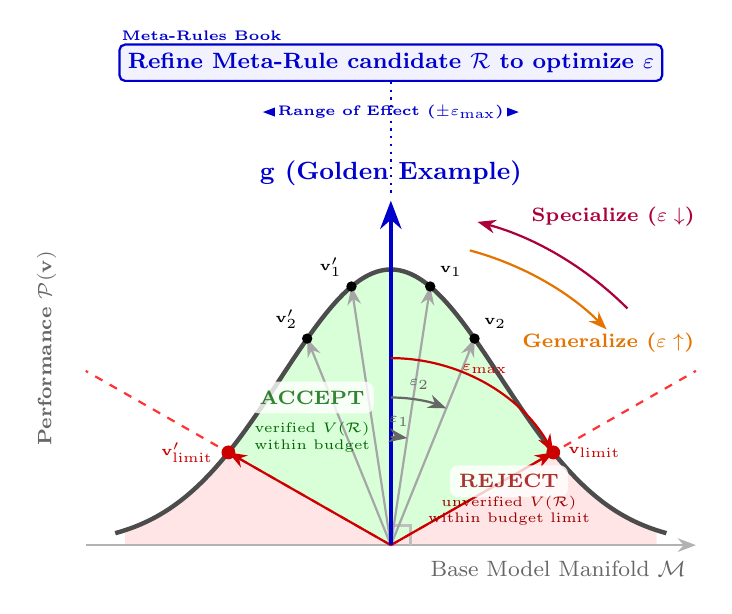
\begin{tikzpicture}[scale=1.25, >=Stealth]

% ---------------- 1. BACKGROUND FILLS (Z-order: Bottom) ----------------
% Acceptance region (Green tint)
\path[fill=green!15]
  (0,0) -- (-1.65, 0.942) -- 
  plot[domain=-1.65:1.65,smooth,samples=100] (\x,{2.8 * exp(-0.4*\x*\x)}) --
  (1.65, 0.942) -- cycle;

% Rejection region (Red tint) - right tail
\path[fill=red!10]
  (0,0) -- (1.65, 0.942) --
  plot[domain=1.65:2.7,smooth,samples=100] (\x,{2.8 * exp(-0.4*\x*\x)}) --
  (2.7, 0) -- cycle;

% Rejection region (Red tint) - left tail
\path[fill=red!10]
  (0,0) -- (-1.65, 0.942) --
  plot[domain=-1.65:-2.7,smooth,samples=100] (\x,{2.8 * exp(-0.4*\x*\x)}) --
  (-2.7, 0) -- cycle;

% ---------------- 2. AXES AND MANIFOLD ----------------
% Base manifold - trimmed to 3.1 to avoid paper edges
\draw[->, thick, gray!60] (-3.1,0) -- (3.1,0) 
  node[anchor=north east, text=gray!80!black, font=\footnotesize, yshift=-2pt] {Base Model Manifold $\mathcal{M}$};

% Perpendicularity marker
\draw[thick, gray!50] (0,0.2) -- (0.2,0.2) -- (0.2,0);

% ---------------- 3. PERFORMANCE LANDSCAPE & BOUNDARIES ----------------
\draw[ultra thick, black!70, domain=-2.8:2.8, smooth, samples=100]
  plot (\x,{2.8 * exp(-0.4*\x*\x)});

% Boundaries
\draw[dashed, red!80, thick] (0,0) -- (3.1, 1.77);
\draw[dashed, red!80, thick] (0,0) -- (-3.1, 1.77);

% ---------------- 4. VECTORS AND DYNAMICS ----------------
\coordinate (V1) at (0.4, 2.627);
\coordinate (V2) at (0.85, 2.098);
\coordinate (Vlim) at (1.65, 0.942);
\coordinate (V1L) at (-0.4, 2.627);
\coordinate (V2L) at (-0.85, 2.098);
\coordinate (VlimL) at (-1.65, 0.942);

% Candidate rays
\draw[->, gray!70, thick] (0,0) -- (V1);
\draw[->, gray!70, thick] (0,0) -- (V2);
\draw[->, red!80!black, thick] (0,0) -- (Vlim);
\draw[->, gray!70, thick] (0,0) -- (V1L);
\draw[->, gray!70, thick] (0,0) -- (V2L);
\draw[->, red!80!black, thick] (0,0) -- (VlimL);

% Intersection markers & Labels
\fill[black] (V1) circle (1.5pt) node[anchor=south west, font=\tiny] {$\mathbf{v}_1$};
\fill[black] (V2) circle (1.5pt) node[anchor=south west, font=\tiny] {$\mathbf{v}_2$};
\fill[red!80!black] (Vlim) circle (2pt) node[anchor=west, font=\tiny, text=red!80!black, xshift=2pt] {$\mathbf{v}_{\text{limit}}$};
\fill[black] (V1L) circle (1.5pt) node[anchor=south east, font=\tiny] {$\mathbf{v}'_1$};
\fill[black] (V2L) circle (1.5pt) node[anchor=south east, font=\tiny] {$\mathbf{v}'_2$};
\fill[red!80!black] (VlimL) circle (2pt) node[anchor=east, font=\tiny, text=red!80!black, xshift=-2pt] {$\mathbf{v}'_{\text{limit}}$};

% Golden Example
\draw[ultra thick, blue!80!black, ->] (0,0) -- (0,3.5);
\node[blue!80!black, anchor=south, font=\small\bfseries] at (0,3.55) {$\mathbf{g}$ (Golden Example)};

% Y-Axis Label (Performance)
\node[rotate=90, anchor=south, font=\scriptsize\bfseries, text=gray!80!black] at (-3.3, 2.0) {Performance $\mathcal{P}(\mathbf{v})$};

% ---------------- 5. META-RULE HEADER ----------------
\coordinate (MetaRule) at (0, 4.9);
\node[draw, blue!80!black, thick, rounded corners=2pt, fill=blue!5, font=\footnotesize\bfseries, inner sep=3pt] (R) at (MetaRule) {Refine Meta-Rule candidate $\mathcal{R}$ to optimize $\varepsilon$};

% Meta-Rules Book label
\node[blue!80!black, font=\tiny\bfseries, anchor=south west, inner sep=1pt] at (R.north west) {Meta-Rules Book};

% Range of Effect line lowered from 4.6 to 4.4
\draw[<->, blue!80!black, thick] (-1.3, 4.4) -- (1.3, 4.4);
\node[blue!80!black, font=\tiny\bfseries, fill=white, inner sep=1pt] at (0, 4.4) {Range of Effect ($\pm\varepsilon_{\max}$)};
\draw[dotted, blue!80!black, thick] (R.south) -- (0, 3.55);

% ---------------- 6. EPSILON ANGLES ----------------
\draw[->, thick, gray!80!black] (0,0) ++(90:1.1) arc (90:81.3:1.1) node[midway, above, font=\tiny] {$\varepsilon_1$};
\draw[->, thick, gray!80!black] (0,0) ++(90:1.5) arc (90:67.9:1.5) node[midway, above, font=\tiny] {$\varepsilon_2$};
\draw[->, thick, red!80!black] (0,0) ++(90:1.9) arc (90:29.7:1.9) node[midway, above, font=\tiny, text=red!80!black] {$\varepsilon_{\max}$};

% ---------------- 7. DIRECTIONAL ARCS (Right Side Stacked & Symmetric) ----------------
% Generalize: Moving AWAY from center (clockwise direction)
% Pointing to the letter 'z' in "Generalize"
\draw[->, thick, orange!90!black] (75:3.1) arc (75:45:3.1);
\node[orange!90!black, font=\scriptsize\bfseries, anchor=west, xshift=-3.4em, yshift=-1.1ex] 
  at (45:3.1) {Generalize ($\varepsilon \uparrow$)};

% Specialize: Moving TOWARD center (counter-clockwise direction)
% Shifted more to the right and kept slightly downward
\draw[->, thick, purple!90!black] (45:3.4) arc (45:75:3.4);
\node[purple!90!black, font=\scriptsize\bfseries, anchor=south west, xshift=1.6em, yshift=-1.2ex] 
  at (75:3.4) {Specialize ($\varepsilon \downarrow$)};

% ---------------- 8. REGION LABELS ----------------
% Accept label: Header at y=1.5, Comment at y=1.1
\node[green!40!black, font=\scriptsize\bfseries, fill=white, fill opacity=0.8, rounded corners=3pt] 
  at (-0.8, 1.5) {ACCEPT};
\node[green!40!black, font=\fontsize{5}{6}\selectfont, align=center] 
  at (-0.8, 1.1) {verified $V(\mathcal{R})$ \\ within budget};

% Reject label: Shifted to (1.2, 0.65) and (1.2, 0.35) to clear the horizontal axis (y=0)
\node[red!60!black, font=\scriptsize\bfseries, fill=white, fill opacity=0.8, rounded corners=3pt] 
  at (1.2, 0.65) {REJECT};
\node[red!60!black, font=\fontsize{5}{6}\selectfont, align=center] 
  at (1.2, 0.35) {unverified $V(\mathcal{R})$ \\ within budget limit};

\end{tikzpicture}
}
\caption{Practically verified semantic cone for supervised Meta-Rule refinement. A golden example direction $\mathbf{g}$ anchors the accepted region. A candidate direction $\mathbf{v}_i$ is screened by a distance such as $d_{\cos}=1-\cos(\angle(\mathbf{v}_i,\mathbf{g}))$ and is applied only when $d_{\cos}\le\epsilon$; it is retained only if the resulting GUMBO contract verifies within the budget. The accepted region therefore represents budget-verifiable generalization, while the rejected region corresponds to semantic or toolchain mismatch.}
\label{fig:vsc}
\vspace{-0.6em}
\end{figure}

\subsubsection{Toy Example Meta-Rule}
Listing~\ref{list:metaRules} shows a compact excerpt from the GUMBO FSE Rule book. The rule directs the agent to introduce explicit GUMBO state when the English requirement implies memory, a failure mode observed in the prompt-only baseline.

\begin{lstlisting}[caption={Compact FSE rule excerpt linking linguistic, semantic, structural, and repair patterns.}, label={list:metaRules}]
Rule: introduce explicit GUMBO state for memory.
Trigger: hysteresis, "hold previous", "shall not change".
Semantic choice: model memory as state + initialization.
Structural target: attach compute_cases to owning SysML thread.
Repair gate: keep only if HAMR/Slang/Logika checks succeed.
\end{lstlisting}

\section{Supervised Meta-Rule Self-Adaptation (Learning) and Acceptance Criteria}
\label{sec:meta-learning}
\subsection{The Algorithm}
\label{sec:algorithm-loop}
Algorithm~\ref{alg:meta-rules} introduces a dual-phase neuro-symbolic process. Let $R$ denote the target set of natural-language requirements, and let $\textsc{Sample}(R)\subset R$ denote the sampled training subset used in developer mode during Phase~I---in our setting, its size was 1/6 of $R$. Let $G=\{(r_g,g_g)\}$ denote the set of golden examples, where $r_g$ is a golden requirement and $g_g$ is its verified formalized GUMBO contract. Let $M$ denote the retained Meta-Rule library, $C$ the set of verified contracts, and $F$ the set of flagged failures.

\textbf{Phase I: Meta-Rule extraction, sample-based training, and predictive $\epsilon$-learning.}
For each golden pair $(r_g,g_g)\in G$, \textsc{ExtractRule} derives a candidate Meta-Rule $m$. For each sampled requirement $r\in \textsc{Sample}(R)$, \textsc{ApplyRule} uses $m$ to produce a candidate formalized contract $\hat{g}$. The quantity $\textsc{Distance}(\hat{g},g_g)$ denotes a \emph{semantic} distance between the generated formalized contract and the golden formalized contract, rather than a literal textual comparison. The threshold $\epsilon$ therefore controls the admissible degree of abstraction away from the golden exemplar. The objective is not to drive $\epsilon$ toward zero: if $\epsilon$ is too small, the rule becomes over-specialized and loses reusability; if $\epsilon$ is too large, the rule admits overly broad generations that require excessive repair or fail to verify within budget $B$. Accordingly, in developer mode $\epsilon$ is tuned across repeated calibration attempts to find a satisfactory intermediate value that best balances rule reuse and bounded repair. Verification is performed by $V(\hat{g},B)$, where $B$ is the repair budget in time and tokens for full repair cycles; the verifier returns a Boolean result $ok$ together with feedback $fb$. While \textsc{RepairBudgetRemaining}$(B)$ holds, \textsc{Repair}$(\hat{g},fb,B)$ revises the candidate using verifier feedback. The counter $okCount$ records how many sampled requirements are successfully verified for the candidate rule $m$, and $\tau$ is the minimum acceptance threshold required to retain $m$ in $M$. If performance is unsatisfactory, \textsc{DiscardOrRefineWithHuman}$(m)$ permits human refinement of the rule, of $\epsilon$, or both, and the developer-mode loop repeats.

\textbf{Phase II: held-out validation and rule-guided formalization with bounded repair.}
After Phase~I, the retained pair $(M,\epsilon)$ is evaluated beyond the sampled training subset. In developer mode, the Phase~II loop is instantiated on requirements not used in $\textsc{Sample}(R)$, testing whether the learned Meta-Rules and calibrated threshold $\epsilon$ generalize to unseen requirements while remaining repairable within budget $B$. In user mode, the same rule-guided synthesis procedure is applied to the full deployment set $R$. For each requirement $r$, \textsc{SynthesizeWithRules}$(r,M)$ produces a candidate contract $\hat{g}$, which is checked again by $V(\hat{g},B)$ and, if needed, revised by \textsc{Repair}$(\hat{g},fb,B)$ while budget remains. If verification succeeds, the pair $(r,\hat{g})$ is added to $C$; otherwise the tuple $(r,\hat{g},fb)$ is added to $F$. Operationally, the developer-mode loop (Phase I and Phase II) repeats until a satisfactory $\epsilon$ is found, namely one for which the retained Meta-Rule library remains reusable on unseen requirements within the available repair budget.

\setlength{\textfloatsep}{8pt}\setlength{\intextsep}{8pt}
\begin{algorithm}[!t]
\caption{SCP Meta-Rules Learning, Application, and Verification-Guided Repair}
\label{alg:meta-rules}
\KwIn{Requirements set $R$; golden examples $G$ (English + formalized GUMBO); verifier $V$ (HAMR/Logika); budgets $B$ (time/tokens/repair cycles); similarity threshold $\epsilon$; acceptance threshold $\tau$.}
\KwOut{Verified contracts $C$; retained Meta-Rules library $M$; flagged failures $F$.}

\textbf{Initialization:}\\
$M \leftarrow \emptyset$ \tcp*{persistent rule memory}
$C \leftarrow \emptyset$; $F \leftarrow \emptyset$\\

\BlankLine
\textbf{Phase I: Meta-Rule extraction and validation}\\
\ForEach{$(r_g, g_g) \in G$}{
  $m \leftarrow \textsc{ExtractRule}(r_g, g_g)$\;
  $okCount \leftarrow 0$\;
  \ForEach{$r \in \textsc{Sample}(R)$}{
    $\hat{g} \leftarrow \textsc{ApplyRule}(m, r)$\;
    \If{$\textsc{Distance}(\hat{g}, g_g) > \epsilon$}{\textbf{continue}\;}
    $(ok, fb) \leftarrow V(\hat{g}, B)$\;
    \While{\textnormal{not} $ok$ \textbf{and} \textsc{RepairBudgetRemaining}$(B)$}{
      $\hat{g} \leftarrow \textsc{Repair}(\hat{g}, fb, B)$\;
      $(ok, fb) \leftarrow V(\hat{g}, B)$\;
    }
    \If{$ok$}{$okCount \leftarrow okCount + 1$\;}
  }
  \eIf{$okCount \ge \tau$}{
    $M \leftarrow M \cup \{m\}$ \tcp*{retain only if it verifies and generalizes}
  }{
    \textsc{DiscardOrRefineWithHuman}$(m)$\;
  }
}

\BlankLine
\textbf{Phase II: Rule-guided formalization with bounded repair}\\
\ForEach{$r \in R$}{
  $\hat{g} \leftarrow \textsc{SynthesizeWithRules}(r, M)$\;
  $(ok, fb) \leftarrow V(\hat{g}, B)$\;
  \While{\textnormal{not} $ok$ \textbf{and} \textsc{RepairBudgetRemaining}$(B)$}{
    $\hat{g} \leftarrow \textsc{Repair}(\hat{g}, fb, B)$\;
    $(ok, fb) \leftarrow V(\hat{g}, B)$\;
  }
  \eIf{$ok$}{
    $C \leftarrow C \cup \{(r,\hat{g})\}$\;
  }{
    $F \leftarrow F \cup \{(r,\hat{g},fb)\}$\;
  }
}

\BlankLine
\textbf{Quality assessment and logging:}\\
Log timestamps, token usage, latency, and repair count; store $M$ for reuse.

\end{algorithm}

\subsection{Scoped GUMBO Rule Book and Function Templates}
\label{sec:gumbo-fse-book}
The evaluated Meta-Rule artifact is the single GUMBO-centered Formal Specification Engineer rule book, referred to here as the \emph{GUMBO FSE Rule book}. We use it as the retained library $M$ in Algorithm~\ref{alg:meta-rules}; broader rule books are excluded from the quantitative evaluation and left to future work. Although the book mainly targets GUMBO formalization, it is toolchain-aware: retained rules record SysML v2 attachment, naming consistency, generated Slang/Scala compatibility, and HAMR/Logika repair cues. The book was extracted/refined from a small solved GUMBO file/subsystem example and then applied to the remaining Monitor/Regulate target files. 
\begin{lstlisting}[caption={Compact ExtractRule, ApplyRule, and Repair templates from the goal files.}, label={list:extract-apply}, basicstyle=\ttfamily\scriptsize]
ExtractRule(req, golden, log):
  record trigger, formal pattern, target construct
  attach SysML/GUMBO placement, naming, Slang,
    verifier expectations, repair_hints, confidence
  return auditable Meta-Rule record

ApplyRule(rule_book, req, active_model):
  load frozen GUMBO FSE rules and active context only
  if semantic_distance(req, rule) > epsilon: flag
  emit GUMBO state/init/compute_cases on owner thread
  report rule ids, ambiguities, checks; run HAMR/Logika

Repair(candidate, feedback, budget):
  classify syntax/attachment/name/type/Slang/Logika error
  minimally edit SysML/GUMBO; do not weaken contracts
  rerun verifier while budget remains; return ok/failure
\end{lstlisting}

The complete rule book, extraction/application/repair templates, evaluation logs, and run videos are linked in the supplementary artifact package.\footnote{Artifact placeholders: \texttt{[rule-book]}, \texttt{[templates]}, \texttt{[logs]}, \texttt{[videos]}.}

Listing~\ref{list:extract-apply} gives compact templates adapted from the learning and user-mode goal files. They show the three roles used in Algorithm~\ref{alg:meta-rules}: extract an auditable rule, apply the frozen book to active project context, and repair only the smallest contract/model fragment when verifier feedback requires it.

\subsection{Practical Considerations and Human Governance}
Meta-Rules are stored as local, version-controlled artifacts and supplied to the agent at execution time together with the verification plan. This design keeps adaptation auditable and allows changes to be reviewed, reproduced, and rolled back. While extraction and validation are highly automated, human oversight remains essential to prevent drift and to decide whether a candidate rule is worth retaining. The threshold $\epsilon$ is therefore calibrated as a satisficing engineering operating point rather than as a theoretical maximum: it is accepted once the learned pair $(M,\epsilon)$ achieves the user-required verification performance on unseen requirements within the available budget. Human review remains part of this calibration loop because the final choice of $\epsilon$ reflects trade-offs among generality, verification success, repair effort, and cost.

%====================================================================
\subsection{Comparison to Fine-Tuning and Transient Prompting}
\label{sec:comparison}

This subsection situates Supervised Meta-Rules Adaptation relative to parameter fine-tuning and transient prompting/ICL. Fine-tuning modifies model weights and can yield strong performance, but it requires suitable data, training authorization, compute, and checkpoint governance that are often difficult in aerospace settings. Prompt-only ICL avoids weight updates, and can behave like ``implicit fine-tuning'' during inference~\cite{vonoswald2023transformers}, but its effects are ephemeral: when the context is reset, the learned behavior is lost, encouraging repeated long-context prompting.

Meta-Rules externalize successful ICL behavior into persistent, version-controlled, verifier-gated artifacts. The surrogate-for-fine-tuning claim is therefore operational rather than universal: Meta-Rules retain task specialization without modifying base-model parameters, while preserving inspectability, rollback, and formal verification-gated acceptance. Table~\ref{tab:adaptation-compare} summarizes the comparison.

\begin{table}[!t]
\caption{Qualitative comparison of adaptation mechanisms for high-assurance pipelines.}
\centering
\label{tab:adaptation-compare}
\scriptsize
\begin{tabular}{p{0.30\columnwidth}ccc}
\hline
 & Fine-tuning & Prompting/ICL & Meta-Rules\\
\hline
Persistent across runs & Yes & No & Yes (external) \\
Model weights tuning& Explicit & Implicit & Implicit \\
Cost & High & Med & Low--Med \\
Auditability / review & Low & Low--Med & High \\
Governance / rollback & Low & Low & High \\
Runtime context overhead & Low & High & Low--Med \\
Data / IP constraints & High & Low--Med & Low \\
FV acceptance gates & N/A & N/A & Primary \\
HAMR toolchain reuse & N/A & Ad hoc & Primary \\
\hline
\end{tabular}
\end{table}

The next section defines the Isolette/HAMR benchmark and reports the two evaluation traces used to measure verification coverage, token cost, and HAMR-scoped reuse.

%====================================================================

\section{Experimental Evaluation: The Isolette GUMBO Benchmark}
\label{sec:example}

We use the Isolette infant-incubator system as a system-level HAMR/INSPECTA benchmark rather than an isolated text-to-contract example~\cite{hatcliff2024isolette}. Isolette contains interacting monitor and regulator subsystems, operator-interface behavior, device/sensor/actuator interactions, and multiple SysML v2 specification/library files. It exercises the HAMR assurance path: requirements become SysML v2/GUMBO artifacts, HAMR generates Slang/Scala proof obligations, and Logika/SMT diagnostics drive repair. The quantitative evaluation focuses on one rule book, the GUMBO FSE Rule book; claims are limited to GUMBO-centered, HAMR-toolchain-aware formalization and repair.

\subsection{Experimental Design and Scope}
\textbf{Inputs.} The experiment uses (i) natural-language requirements from a realistic FAA-style source containing text, tables, and figures, and (ii) SysML v2 models/shared libraries for the Isolette architecture, including \texttt{Monitor.sysml} and \texttt{Regulate.sysml}~\cite{lempia2009faa}. These artifacts include terminology, cross-references, and memory-bearing requirements such as hysteresis that must be encoded in tool-accepted GUMBO. Naive repair can replay requirements, model fragments, generated Slang/Scala code, build logs, proof obligations, and counterexamples, producing long-context blow-up across the stack.

\textbf{Scope of evaluation.} The target set contains 42 proof-bearing units: GUMBO contract-bearing blocks, generated or modified \texttt{compute\_cases}, and corresponding HAMR-generated methods checked by Logika for the Monitor/Regulate target. This scope is explicitly bounded, but remains system-level and multi-layered because a GUMBO decision must survive SysML v2 placement, HAMR generation, generated Slang/Scala obligations, and Logika proof discharge.

\textbf{Runs and training split.} We compare a prompt-only baseline with a Meta-Rule run using the GUMBO FSE Rule book at $\epsilon=0.1$. Developer mode extracts/refines the rule book from a small solved GUMBO file/subsystem example, then applies the retained knowledge to the remaining target files. This tests intra-system, cross-subsystem reuse under HAMR/INSPECTA; the reported adjusted trace already includes extraction/refinement and successful verification.

\subsection{Observed Failure and Self-Healing Behavior}
The baseline repeatedly attempted incompatible pre-state idioms for memory-bearing requirements and did not converge on tool-accepted GUMBO state syntax. The Meta-Rule-guided run uses the GUMBO FSE Rule book to introduce explicit state, initialization guarantees, and structured \texttt{compute\_cases}; it also uses toolchain-facing repair cues for SysML attachment, naming consistency, generated Slang/Scala obligations, and HAMR/Logika diagnostics. Listing~\ref{list:failureLog} gives the condensed baseline log; the verified Meta-Rule-guided result and adjusted cost are reported in Table~\ref{tab:results} and Fig.~\ref{fig:results} to avoid duplicating the same cost trace in a separate listing.

\begin{lstlisting}[caption={Condensed baseline failure excerpt: parser rejection and high token usage.}, label={list:failureLog}, float=t]
Baseline: Parser rejected memory idioms:
  "rejects every variant of the state ... syntax"
  "@pre as an unsupported classification test"
Result: could not encode hysteresis/no-change cases.
Tokens: input=981,770 (+18,673,920 cached),
        output=85,833.
\end{lstlisting}

% The success transcript is omitted from the submission version because the
% adjusted cost and verification result are reported in Table~\ref{tab:results}.
%\begin{lstlisting}[caption={Condensed GUMBO FSE Meta-Rule success excerpt: verified target scope.}, label={list:successLog}, float=t]
%GUMBO FSE Rule book: add GUMBO state for last mode,
%INIT timer, previous actuation, hysteresis, and
%REQ_MRM_1--4 / REQ_MHS_1--5 compute cases.
%Verification:
%  sireum hamr sysml logika --sourcepath isolette/sysml
%  isolette/hamr/slang/bin/run-logika.cmd
%Logika proved all tasks successfully for the
%Monitor/Regulate target scope.
%\end{lstlisting}

\subsection{Metrics, Pricing Model, and Results}
\label{sec:evaluation}
The evaluation measures more than final correctness. In a multi-layer HAMR workflow, early formalization errors can propagate into generated implementation artifacts and proof obligations, increasing both the number of repair paths and the amount of context that must be reprocessed. The token, throughput, and adjusted-cost metrics therefore capture whether the copilot reaches verifier-accepted artifacts without allowing stochastic repair to expand beyond the available budget.

For a run $r$, we report wall-clock time $T_{wall}(r)$, uncached input tokens $N_{in}(r)$, cached input tokens $N_{cache}(r)$, and output-side tokens $N_{out}(r)$. We do not separately tabulate reasoning tokens in the main results because the pricing model used here distinguishes input, cached input, and output-side tokens; any separately logged reasoning count is therefore treated as part of the output-side cost discussion rather than as a separate priced class. We define the context-processed total
\begin{equation}
N_{ctx}(r)=N_{in}(r)+N_{cache}(r)+N_{out}(r).
\end{equation}
This distinction matters because current provider pricing differentiates uncached input, cached input, and output tokens.\footnote{Pricing reference used for the model-cost discussion: \url{https://developers.openai.com/api/docs/pricing}. At the time of writing, the illustrative standard Codex price tags used in Table~\ref{tab:results} are $p_{in}=\$60$/M long-context input tokens, $p_{cache}=\$0$/M cached tokens, and $p_{out}=\$270$/M output-side tokens. Prices and thresholds change over time, so the paper reports token classes and symbolic prices rather than treating dollar amounts as invariant.} Let $pm=(p_{in},p_{cache},p_{out})$ denote the selected pricing model. The illustrative dollar cost of a logged run is
\begin{equation}
C(r;pm)=\frac{p_{in}N_{in}(r)+p_{cache}N_{cache}(r)+p_{out}N_{out}(r)}{10^{6}}.
\end{equation}
Because the illustrative pricing model sets $p_{cache}=0$, cached tokens affect context-size and burn-rate metrics but not the dollar estimates in Table~\ref{tab:results}.

\noindent\textbf{Adjusted cost.}
The adjusted trace in Table~\ref{tab:results} is a complete logged run that already includes the one-time developer-mode extraction/refinement effort for the GUMBO FSE Rule book and the successful verification run. Therefore, for that trace we do not add a separate user-mode run again. We define
\begin{equation}
N_{adj}(r)=N_{ctx}(r), \qquad C_{adj}(r;pm)=C(r;pm),
\end{equation}
and report the adjusted per-verified-unit quantities
\begin{equation}
K_{adj}(r)=\frac{N_{adj}(r)}{|U_{verified}(r)|}, \qquad
K_{\$}^{adj}(r)=\frac{C_{adj}(r;pm)}{|U_{verified}(r)|}.
\end{equation}
When developer-mode and later user-mode logs are measured separately, the amortized form for $H$ future reuse opportunities is
\begin{equation}
C_{adj}^{(H)}(r;pm)=C_{use}(r;pm)+\frac{C_{dev}(pm)}{H}.
\end{equation}
This paper reports the more conservative complete adjusted trace for the scoped GUMBO experiment.

Let $U_{verified}(r)\subseteq U$ denote the verified subset of the 42 targeted units. We define
\begin{align}
\rho(r) &= \frac{|U_{verified}(r)|}{|U|}, \\
\Theta(r) &= \frac{|U_{verified}(r)|}{T_{wall}(r)}, \\
K(r) &= \frac{N_{ctx}(r)}{|U_{verified}(r)|}.
\end{align}
For runs with $T_{wall}(r)>0$ and $|U_{verified}(r)|>0$, the context-token burn rate is $\Gamma_{ctx}(r)=N_{ctx}(r)/T_{wall}(r)=K(r)\Theta(r)$. For partial verification, comparisons are defined only over the common target subset, not merely by the number of verified units. Table~\ref{tab:results} reports the adjusted values and Fig.~\ref{fig:results} visualizes the same scoped comparison.

\begin{table*}[!t]
\centering
\caption{Representative adjusted run metrics for the scoped GUMBO evaluation. The adjusted column is a complete logged run, so the one-time extraction/refinement effort is already included. Dollar costs use the current pricing model in the footnote; cached-token price is set to zero in that model.}
\label{tab:results}
\scriptsize
\setlength{\tabcolsep}{3pt}
\begin{tabular}{@{}p{0.33\textwidth}p{0.27\textwidth}p{0.30\textwidth}@{}}
\hline
Metric & Baseline: no Meta-Rules & Adjusted $\epsilon=0.1$: the GUMBO FSE Rule book \\
\hline
Rule-book scope & None & GUMBO-centered FSE rules with toolchain-aware repair \\
Phase reported & Prompt-only user run & Adjusted complete run \\
Training / reuse source & None & One solved/golden GUMBO file/subsystem; evaluated on remaining target files \\
Toolchain layers exercised & SysML/GUMBO attempted; verification fails & SysML v2 placement, GUMBO, generated Slang/Scala obligations, Logika repair \\
Price tags (per M tokens) & input \$60; cached \$0; output \$270 & same \\
$T_{wall}$ (min) & 33 & 39 \\
$N_{in}$ & 981{,}770 & 381{,}624 \\
$N_{cache}$ & 18{,}673{,}920 & 13{,}391{,}360 \\
$N_{out}$ & 85{,}833 & 57{,}821 \\
Logged priced tokens $N_{in}+N_{out}$ & 1{,}067{,}603 & 439{,}445 \\
Final goal usage & -- & 436{,}169 \\
Illustrative $C$ / $C_{adj}$ ($p_{cache}=0$) & $\$82.08$ & $\$38.51$ \\
$N_{ctx}$ & 19{,}741{,}523 & 13{,}830{,}805 \\
$\Gamma_{ctx}$ (tokens/min) & $\approx$598K & $\approx$355K \\
$|U|$ targeted units & \textit{42} & \textit{42} \\
$|U_{verified}|$ & \textit{2} & \textit{42} \\
$\rho$ & \textit{4.76\%} & \textit{100\%} \\
$\Theta$ (units/min) & \textit{0.06} & \textit{1.08} \\
$K$ / $K_{adj}$ (context tokens/verified unit) & $\approx$9.87M & $\approx$329K \\
$K_{\$}$ / $K_{\$}^{adj}$ (dollars/verified unit) & $\$41.04$ & $\$0.92$ \\
$S$ (end-to-end success) & 0 & 1 \\
\hline
\end{tabular}
\end{table*}

\begin{figure*}[!t]
\centering
\resizebox{0.88\textwidth}{!}{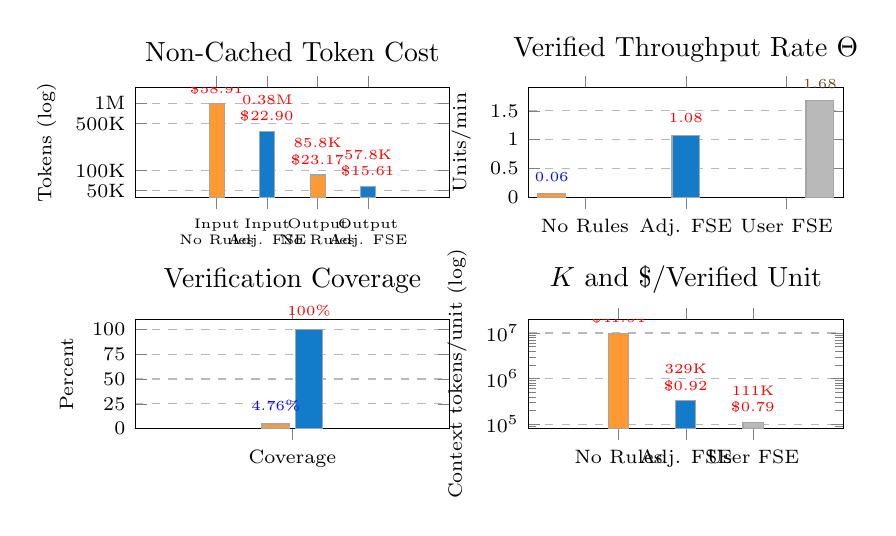
\begin{tikzpicture}
\begin{groupplot}[
  group style={group size=2 by 2, horizontal sep=1.00cm, vertical sep=1.55cm},
  width=0.46\textwidth,
  height=0.245\textwidth,
  ymajorgrids=true,
  grid style={dashed, gray!55},
  tick label style={font=\scriptsize},
  label style={font=\scriptsize},
  title style={font=\normalsize},
  legend style={font=\scriptsize, draw=gray!25, fill=white, at={(0.02,0.98)}, anchor=north west, legend cell align=left},
  ybar,
  x tick label style={rotate=0, anchor=north, font=\scriptsize, align=center},
  enlarge x limits=0.28,
  nodes near coords,
  every node near coord/.append style={font=\tiny, yshift=1pt},
  point meta=explicit symbolic,
]



\nextgroupplot[
  title={Non-Cached Token Cost},
  ylabel={Tokens (log)},
  ymode=log,
  log basis y=10,
  ymin=0.04, ymax=1.7,
  xmin=0.5, xmax=4.5,
  xtick={1,2,3,4},
  xticklabels={Input\\No Rules,Input\\Adj. FSE,Output\\No Rules,Output\\Adj. FSE},
  ytick={0.05,0.1,0.5,1},
  yticklabels={50K,100K,500K,1M},
  x tick label style={rotate=0, anchor=north, font=\tiny, align=center},
  nodes near coords=false,
]
\draw[draw=black!35, fill=orange!80] (axis cs:0.85,0.04) rectangle (axis cs:1.15,0.982);
\node[font=\tiny, text=red, anchor=south, align=center] at (axis cs:1,0.982) {0.98M\\\$58.91};
\draw[draw=black!35, fill=cyan!60!blue] (axis cs:1.85,0.04) rectangle (axis cs:2.15,0.382);
\node[font=\tiny, text=red, anchor=south, align=center] at (axis cs:2,0.382) {0.38M\\\$22.90};
\draw[draw=black!35, fill=orange!80] (axis cs:2.85,0.04) rectangle (axis cs:3.15,0.0858);
\node[font=\tiny, text=red, anchor=south, align=center] at (axis cs:3,0.0858) {85.8K\\\$23.17};
\draw[draw=black!35, fill=cyan!60!blue] (axis cs:3.85,0.04) rectangle (axis cs:4.15,0.0578);
\node[font=\tiny, text=red, anchor=south, align=center] at (axis cs:4,0.0578) {57.8K\\\$15.61};


\nextgroupplot[
  title={Verified Throughput Rate $\Theta$},
  ylabel={Units/min},
  symbolic x coords={Base,Adjusted,User},
  xtick={Base,Adjusted,User},
  xticklabels={No Rules,Adj. FSE,User FSE},
  ymin=0, ymax=1.9,
  ytick={0,0.5,1.0,1.5},
  nodes near coords,
]
\addplot+[draw=black!35, fill=orange!80] coordinates {(Base,0.06) [0.06]};
\addplot+[draw=black!35, fill=cyan!60!blue] coordinates {(Adjusted,1.08) [1.08]};
\addplot+[draw=black!35, fill=gray!55] coordinates {(User,1.68) [1.68]};

\nextgroupplot[
  title={Verification Coverage},
  ylabel={Percent},
  symbolic x coords={Coverage},
  xtick=data,
  ymin=0, ymax=110,
  ytick={0,25,50,75,100},
  x tick label style={rotate=0, anchor=north, font=\scriptsize},
]
\addplot+[draw=black!35, fill=orange!80] coordinates {(Coverage,4.76) [4.76\%]};
\addplot+[draw=black!35, fill=cyan!60!blue] coordinates {(Coverage,100) [100\%]};

\nextgroupplot[
  title={$K$ and \$/Verified Unit},
  ylabel={Context tokens/unit (log)},
  ymode=log,
  log basis y=10,
  ymin=8e4, ymax=2e7,
  xmin=0.5, xmax=3.5,
  xtick={1,2,3},
  xticklabels={No Rules,{Adj. FSE},{User FSE}},
  x tick label style={rotate=0, anchor=north, font=\scriptsize, align=center},
  nodes near coords=false,
]
\draw[draw=black!35, fill=orange!80] (axis cs:0.85,8e4) rectangle (axis cs:1.15,9.87e6);
\node[font=\tiny, text=red, anchor=south, align=center] at (axis cs:1,9.87e6) {9.87M\\\$41.04};
\draw[draw=black!35, fill=cyan!60!blue] (axis cs:1.85,8e4) rectangle (axis cs:2.15,3.29e5);
\node[font=\tiny, text=red, anchor=south, align=center] at (axis cs:2,3.29e5) {329K\\\$0.92};
\draw[draw=black!35, fill=gray!55] (axis cs:2.85,8e4) rectangle (axis cs:3.15,1.11e5);
\node[font=\tiny, text=red, anchor=south, align=center] at (axis cs:3,1.11e5) {111K\\\$0.79};

\end{groupplot}
\end{tikzpicture}
}
\caption{Adjusted quantitative comparison for the scoped Isolette/GUMBO FSE evaluation. The chart uses the same baseline and adjusted $\epsilon=0.1$ trace as Table~\ref{tab:results}. The first panel shows only the non-cached priced token classes, input and output, with the same style of dollar tags used in the cost panel; cached tokens are still reported in Table~\ref{tab:results} because they affect context size but have zero cost in the illustrative pricing model. The throughput panel reports $\Theta$ for baseline, adjusted complete run, and the later user-mode run after the rule book exists; the cost panel reports $K$ and dollar cost per verified unit.}
\label{fig:results}
\vspace{-0.6em}
\end{figure*}

\noindent\textbf{Interpretation.}
 Table~\ref{tab:results} reports the adjusted cost for the evaluated Meta-Rule condition, and Fig.~\ref{fig:results} restores the visual comparison for the same scoped traces. The adjusted $\epsilon=0.1$ trace includes the one-time extraction/refinement effort for the GUMBO FSE Rule book and the successful verification run in the same logged trace. Even without amortizing that one-time investment across future uses, the Meta-Rule-guided trace reduces cost per verified unit from $\approx9.87$M to $\approx329$K context tokens and from $\$41.04$ to $\$0.92$ in the illustrative pricing model. The later user-mode run, after the rule book exists, gives the usage-phase throughput reference $\Theta=1.68$ units/min; the adjusted complete run gives the more conservative $\Theta=1.08$ units/min after including the one-time effort. %At this stage of our research, the important learning claim is deliberately scoped: a small solved formalization example provides reusable HAMR/INSPECTA repair knowledge for the remaining target files in the same system.% The previously reported 28$\times$ throughput improvement is therefore qualified as a usage-phase observation after the rule book exists; the adjusted table reports the conservative complete-run comparison for the scoped GUMBO case.


\section{Related Work}
\label{sec:related-work}

LLMs have increasingly been used to assist formal reasoning and proof engineering. GPT-f explored generative theorem proving in Metamath~\cite{polu2020generative}, while Baldur and CoqDog-style systems study whole-proof generation, repair, and diagnosis in proof assistants such as Isabelle/HOL and Coq~\cite{first2023baldur,CoqDog}. Other neuro-symbolic and verification-oriented workflows integrate LLMs with code verification, SMT-backed checks, or symbolic reasoning benchmarks~\cite{DBLP:conf/popl/SwamyHKRDFBFSKZ16,aws_bedrock_ar,mirzadeh2025gsmsymbolic}. These efforts are adjacent because they combine LLMs with formal structure, but they typically operate at a proof-script, theorem-proving, requirements-auditing, or code-verification layer.

Formal methods are also being integrated into MBSE standards and tools. SysML v2 was designed with formal semantics in mind~\cite{sysmlv2}, and Imandra has demonstrated model-level SysML v2 verification~\cite{imandra_sysml}. AGREE-Dog is the closest MBSE copilot because it supports AADL/AGREE model-level explanation and repair~\cite{agreedog_tahat2025,feiler-aadl}. SCP differs in its evaluated boundary: the GUMBO FSE Rule book must help produce contracts that are placed in SysML v2, preserved through HAMR generation, reflected in generated Slang/Scala obligations, and discharged by Logika. The learned object is therefore not merely a prompt hint or proof tactic, but a HAMR-centric memory of linguistic triggers, semantic GUMBO choices, structural placement decisions, and verifier-guided repair actions.
\section{Limitations and Future Work}
\label{sec:limitations}

Our evaluation is conducted on the Isolette infant-incubator system~\cite{hatcliff2024isolette},
a realistic multi-subsystem HAMR/INSPECTA benchmark that exercises natural-language
requirements, SysML v2 modeling, GUMBO contract synthesis, HAMR-generated
Slang/Scala proof obligations, and Logika proof discharge. Within this benchmark,
our methodology demonstrates that reusable formalization and repair knowledge can
be learned from a small set of solved file- and subsystem-level examples and then
applied to support verification of remaining target files. In particular, our approach
converted a prompt-only failure into an end-to-end fully verified target-scope run,
while substantially reducing cost and time. This is a significant result given that
direct fine-tuning of the base model was restricted.

The current evaluation is intentionally scoped to toolchain-aware GUMBO
formalization and repair for the Isolette/HAMR target. Broader validation remains
future work. We plan to evaluate additional HAMR rule books for SysML synthesis,
Rust/Verus repair, and other high-assurance systems, including seL4-based firewall
architectures~\cite{Hatcliff:seL4Summit2025}. We will also investigate repair
heuristics inspired by \textsc{VeriStruct}~\cite{sun2025veristruct}, cloud-scale
verification, multimodal specification, and advances in compositional reasoning for
GUMBO/AGREE~\cite{compositional-analysis-agree,agreedog_tahat2025}.

%====================================================================
\section{Conclusion}
\label{sec:conclusion}

This paper presents SCP as a practical methodology for converting transient LLM
formalization behavior into reusable engineering knowledge within a HAMR/INSPECTA
workflow. Rather than treating learned information as informal prompt hints or
isolated proof tactics, our approach organizes it as auditable rules that connect
linguistic requirement triggers, semantic GUMBO choices, SysML v2 placement,
generated Slang/Scala obligations, and Logika feedback. This provides a practical
adaptation mechanism for high-assurance model-based engineering workflows even
when direct fine-tuning is unavailable.

The Isolette benchmark illustrates the value of this approach. A naive agentic
workflow may repeatedly replay requirements, SysML v2 models, GUMBO contracts,
generated code, proof obligations, logs, and counterexamples until token and repair
budgets are exhausted. By contrast, the GUMBO FSE Rule Book enabled our workflow
to compact recurring formalization and repair knowledge, turning a failing
prompt-only run into a fully verified target-scope run while saving millions of
context tokens relative to the baseline. These results provide encouraging evidence
that our appraoch can improve reliable verified throughput in high-assurance realistic HAMR model based system engineering.

Overall, our methodology points toward a practical integration pattern for GenAI in
high-assurance engineering: auditable learned rules, bounded self-healing, and
formal verification as the primary acceptance gate.


\section*{Acknowledgment}
This work was funded by DARPA contract FA8750-24-9-1000. The views, opinions, and/or findings expressed are those of the authors and should not be interpreted as representing the official views or policies of DARPA, the U.S. Department of Defense, or the U.S. Government. 

%====================================================================
% Appendices removed for the 10-page IEEE submission.
% They can be restored for the Loonwerks extended version.
\iffalse
%\appendices
%====================================================================
%====================================================================
\appendices

\section{Geometric and Performance Interpretation of Meta-Rule }
\label{app:vsc}

This appendix extends the geometric interpretation of the Meta-Rule methodology by introducing a verification-aligned performance landscape over the embedding space. The resulting view clarifies how semantic generalization, formal verification constraints, and computational budget jointly determine admissible generations in the SCP workflow.

\subsection{Embedding-Space Abstraction}

Let $\mathcal{M} \subset \mathbb{R}^d$ denote the latent embedding manifold induced by a pretrained base model. Let $\mathbf{g} \in \mathbb{R}^d$ represent the embedding of a \emph{golden example}, corresponding to a formally verified transformation:
\[
\text{English requirement}
\rightarrow
\text{SysML v2 + GUMBO}
\rightarrow
\text{HAMR}~\text{code}\]
\[\rightarrow
\text{Logika proof discharge}.
\]
For conceptual clarity, we depict the base model’s prior generative tendency as a horizontal manifold, while the golden example $\mathbf{g}$ is shown as a perpendicular semantic direction. This orthogonality is interpretive: it emphasizes that the golden example represents a correctness-anchored direction relative to unconstrained generation.

Under a Meta-Rule set $\mathcal{R}_i$, the SCP copilot produces a candidate embedding
\begin{equation}
\mathbf{v}_i = f_{\theta,\mathcal{R}_i}(x),
\end{equation}
where $f_{\theta}$ is the base model and $x$ is the input requirement. The semantic deviation from the golden example is quantified by
\begin{equation}
\varepsilon_i = \angle(\mathbf{v}_i,\mathbf{g}).
\end{equation}
The parameter $\varepsilon_i$ reflects controlled abstraction away from the exemplar.

\subsection{Practically Verified Semantic Cone and Budgeted Acceptance}

Meta-Rules constrain the effective sampling region of the model. Geometrically, admissible candidates form a conical neighborhood around $\mathbf{g}$. Let
\[
V(\mathbf{v}_i)\in\{0,1\}
\]
denote the outcome of integration-level and code-level Logika verification under a bounded computational budget and humain review (tokens, repair cycles, and time constraints). A candidate is accepted if and only if:
\begin{equation}
V(\mathbf{v}_i)=1.
\end{equation}
The admissible region defines a \emph{Practically Verified Semantic Cone}: the maximal angular neighborhood around $\mathbf{g}$ within which artifacts remain formally verifiable under the design budget. Outside this cone lies a \emph{rejection region}---generations that either (i) violate logical constraints or (ii) require repair effort exceeding the verification budget. Thus, rejection is not merely semantic divergence but \emph{budget-constrained unverifiability} %(Edit this: i.e., it will be practically be expensive to repair the generated models within a given budget).

\subsection{Performance Landscape and Token-Accounted Outcomes}

We further interpret the embedding space as supporting a scalar performance functional $\mathcal{P}(\mathbf{v})$ that captures verification-aligned utility (e.g., semantic alignment to the golden exemplar, syntactic/tool compatibility, and repair efficiency). In Fig.~\ref{fig:vsc}, $\mathcal{P}$ is depicted as a bell-shaped (local maximum) curve centered near the golden example direction. Each ray denotes a candidate generation direction $\mathbf{v}_i$; its intersection with the performance curve yields an observed outcome point (dot) whose associated token-accounting vector summarizes execution cost:
\[
\mathbf{t}_i =
\begin{bmatrix}
N_{\mathrm{in}} \\
N_{\mathrm{cache}} \\
N_{\mathrm{reason}} \\
N_{\mathrm{total}}
\end{bmatrix},
\]
where $N_{\mathrm{in}}$ is uncached input tokens, $N_{\mathrm{cache}}$ is cached input tokens, $N_{\mathrm{reason}}$ is reasoning tokens, and $N_{\mathrm{total}}$ is total tokens.

The \emph{acceptance region} is the high-performance basin enclosed by the cone and the performance curve, where candidates remain verifiable under the design budget. The \emph{rejection region} is the region bounded by the lower cone edge, the baseline, and the performance curve; candidates falling into this region are practically formally unverifiable within the allocated verification/repair budget.
%\appendices

%\section{Geometric and Performance Interpretation of Meta-Rule Generalization}
%\label{app:vsc}

%This appendix extends the geometric interpretation of the Meta-Rule methodology by introducing a verification-aligned performance landscape over the embedding space.

\begin{figure}[h]
\centering
%\begin{figure}[htbp]
%\centering
% Scale 1.25 ensures horizontal clearance within margins
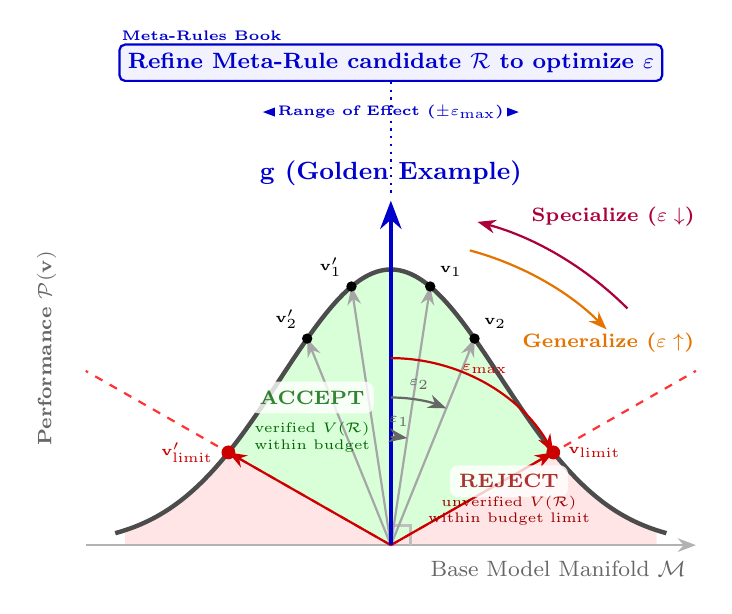
\begin{tikzpicture}[scale=1.25, >=Stealth]

% ---------------- 1. BACKGROUND FILLS (Z-order: Bottom) ----------------
% Acceptance region (Green tint)
\path[fill=green!15]
  (0,0) -- (-1.65, 0.942) -- 
  plot[domain=-1.65:1.65,smooth,samples=100] (\x,{2.8 * exp(-0.4*\x*\x)}) --
  (1.65, 0.942) -- cycle;

% Rejection region (Red tint) - right tail
\path[fill=red!10]
  (0,0) -- (1.65, 0.942) --
  plot[domain=1.65:2.7,smooth,samples=100] (\x,{2.8 * exp(-0.4*\x*\x)}) --
  (2.7, 0) -- cycle;

% Rejection region (Red tint) - left tail
\path[fill=red!10]
  (0,0) -- (-1.65, 0.942) --
  plot[domain=-1.65:-2.7,smooth,samples=100] (\x,{2.8 * exp(-0.4*\x*\x)}) --
  (-2.7, 0) -- cycle;

% ---------------- 2. AXES AND MANIFOLD ----------------
% Base manifold - trimmed to 3.1 to avoid paper edges
\draw[->, thick, gray!60] (-3.1,0) -- (3.1,0) 
  node[anchor=north east, text=gray!80!black, font=\footnotesize, yshift=-2pt] {Base Model Manifold $\mathcal{M}$};

% Perpendicularity marker
\draw[thick, gray!50] (0,0.2) -- (0.2,0.2) -- (0.2,0);

% ---------------- 3. PERFORMANCE LANDSCAPE & BOUNDARIES ----------------
\draw[ultra thick, black!70, domain=-2.8:2.8, smooth, samples=100]
  plot (\x,{2.8 * exp(-0.4*\x*\x)});

% Boundaries
\draw[dashed, red!80, thick] (0,0) -- (3.1, 1.77);
\draw[dashed, red!80, thick] (0,0) -- (-3.1, 1.77);

% ---------------- 4. VECTORS AND DYNAMICS ----------------
\coordinate (V1) at (0.4, 2.627);
\coordinate (V2) at (0.85, 2.098);
\coordinate (Vlim) at (1.65, 0.942);
\coordinate (V1L) at (-0.4, 2.627);
\coordinate (V2L) at (-0.85, 2.098);
\coordinate (VlimL) at (-1.65, 0.942);

% Candidate rays
\draw[->, gray!70, thick] (0,0) -- (V1);
\draw[->, gray!70, thick] (0,0) -- (V2);
\draw[->, red!80!black, thick] (0,0) -- (Vlim);
\draw[->, gray!70, thick] (0,0) -- (V1L);
\draw[->, gray!70, thick] (0,0) -- (V2L);
\draw[->, red!80!black, thick] (0,0) -- (VlimL);

% Intersection markers & Labels
\fill[black] (V1) circle (1.5pt) node[anchor=south west, font=\tiny] {$\mathbf{v}_1$};
\fill[black] (V2) circle (1.5pt) node[anchor=south west, font=\tiny] {$\mathbf{v}_2$};
\fill[red!80!black] (Vlim) circle (2pt) node[anchor=west, font=\tiny, text=red!80!black, xshift=2pt] {$\mathbf{v}_{\text{limit}}$};
\fill[black] (V1L) circle (1.5pt) node[anchor=south east, font=\tiny] {$\mathbf{v}'_1$};
\fill[black] (V2L) circle (1.5pt) node[anchor=south east, font=\tiny] {$\mathbf{v}'_2$};
\fill[red!80!black] (VlimL) circle (2pt) node[anchor=east, font=\tiny, text=red!80!black, xshift=-2pt] {$\mathbf{v}'_{\text{limit}}$};

% Golden Example
\draw[ultra thick, blue!80!black, ->] (0,0) -- (0,3.5);
\node[blue!80!black, anchor=south, font=\small\bfseries] at (0,3.55) {$\mathbf{g}$ (Golden Example)};

% Y-Axis Label (Performance)
\node[rotate=90, anchor=south, font=\scriptsize\bfseries, text=gray!80!black] at (-3.3, 2.0) {Performance $\mathcal{P}(\mathbf{v})$};

% ---------------- 5. META-RULE HEADER ----------------
\coordinate (MetaRule) at (0, 4.9);
\node[draw, blue!80!black, thick, rounded corners=2pt, fill=blue!5, font=\footnotesize\bfseries, inner sep=3pt] (R) at (MetaRule) {Refine Meta-Rule candidate $\mathcal{R}$ to optimize $\varepsilon$};

% Meta-Rules Book label
\node[blue!80!black, font=\tiny\bfseries, anchor=south west, inner sep=1pt] at (R.north west) {Meta-Rules Book};

% Range of Effect line lowered from 4.6 to 4.4
\draw[<->, blue!80!black, thick] (-1.3, 4.4) -- (1.3, 4.4);
\node[blue!80!black, font=\tiny\bfseries, fill=white, inner sep=1pt] at (0, 4.4) {Range of Effect ($\pm\varepsilon_{\max}$)};
\draw[dotted, blue!80!black, thick] (R.south) -- (0, 3.55);

% ---------------- 6. EPSILON ANGLES ----------------
\draw[->, thick, gray!80!black] (0,0) ++(90:1.1) arc (90:81.3:1.1) node[midway, above, font=\tiny] {$\varepsilon_1$};
\draw[->, thick, gray!80!black] (0,0) ++(90:1.5) arc (90:67.9:1.5) node[midway, above, font=\tiny] {$\varepsilon_2$};
\draw[->, thick, red!80!black] (0,0) ++(90:1.9) arc (90:29.7:1.9) node[midway, above, font=\tiny, text=red!80!black] {$\varepsilon_{\max}$};

% ---------------- 7. DIRECTIONAL ARCS (Right Side Stacked & Symmetric) ----------------
% Generalize: Moving AWAY from center (clockwise direction)
% Pointing to the letter 'z' in "Generalize"
\draw[->, thick, orange!90!black] (75:3.1) arc (75:45:3.1);
\node[orange!90!black, font=\scriptsize\bfseries, anchor=west, xshift=-3.4em, yshift=-1.1ex] 
  at (45:3.1) {Generalize ($\varepsilon \uparrow$)};

% Specialize: Moving TOWARD center (counter-clockwise direction)
% Shifted more to the right and kept slightly downward
\draw[->, thick, purple!90!black] (45:3.4) arc (45:75:3.4);
\node[purple!90!black, font=\scriptsize\bfseries, anchor=south west, xshift=1.6em, yshift=-1.2ex] 
  at (75:3.4) {Specialize ($\varepsilon \downarrow$)};

% ---------------- 8. REGION LABELS ----------------
% Accept label: Header at y=1.5, Comment at y=1.1
\node[green!40!black, font=\scriptsize\bfseries, fill=white, fill opacity=0.8, rounded corners=3pt] 
  at (-0.8, 1.5) {ACCEPT};
\node[green!40!black, font=\fontsize{5}{6}\selectfont, align=center] 
  at (-0.8, 1.1) {verified $V(\mathcal{R})$ \\ within budget};

% Reject label: Shifted to (1.2, 0.65) and (1.2, 0.35) to clear the horizontal axis (y=0)
\node[red!60!black, font=\scriptsize\bfseries, fill=white, fill opacity=0.8, rounded corners=3pt] 
  at (1.2, 0.65) {REJECT};
\node[red!60!black, font=\fontsize{5}{6}\selectfont, align=center] 
  at (1.2, 0.35) {unverified $V(\mathcal{R})$ \\ within budget limit};

\end{tikzpicture}

\caption{
Verified Semantic Cone with a bell-shaped verification-aligned performance landscape $\mathcal{P}(\mathbf{v})$ for supervised Meta-Rule refinement. The golden example direction $\mathbf{g}$ (blue) is perpendicular to the base model manifold $\mathcal{M}$. Under a Meta-Rule candidate $\mathcal{R}$, generated candidates (rays) intersect $\mathcal{P}$ at outcome points $\mathbf{v}_i$. Clockwise increases in $\varepsilon$ promote generalization ($\varepsilon\uparrow$), while counterclockwise decreases promote specialization ($\varepsilon\downarrow$). The range of effect ($\pm\varepsilon_{\max}$) and boundary points $\mathbf{v}_{\text{limit}}$ separate the accepted region (green, verified $V(\mathcal{R})$ within budget) from the rejected region (red, unverified within the budget limit). Increasing $\varepsilon$ expands the neighborhood in which $\mathcal{R}$ yields semantically correct, practically verifiable formalizations, enabling a small number of golden examples (e.g., one GUMBO block) to generalize to a larger class of verified contracts through semantic (not merely syntactic) refinement.
%Verified Semantic Cone with a bell-shaped verification-aligned performance landscape $\mathcal{P}(\mathbf{v})$ for supervised Meta-Rule refinement. The golden example direction $\mathbf{g}$ (blue) is perpendicular to the base model manifold $\mathcal{M}$. Under a Meta-Rule candidate $\mathcal{R}$, generated candidates (rays) intersect $\mathcal{P}$ at outcome points $\mathbf{v}_i$. Clockwise increases in $\varepsilon$ promote generalization ($\varepsilon\uparrow$), while counterclockwise decreases promote specialization ($\varepsilon\downarrow$). The range of effect ($\pm\varepsilon_{\max}$) and boundary points $\mathbf{v}_{\text{limit}}$ separate the accepted region (green, verified $V(\mathcal{R})$ within budget) from the rejected region (red, unverified within the budget limit).
%Verified Semantic Cone with a bell-shaped verification-aligned performance landscape $\mathcal{P}(\mathbf{v})$. The golden example direction $\mathbf{g}$ is shown perpendicular to the base model manifold. Rays represent candidate generations $\mathbf{v}_i$; their intersections (dots) with $\mathcal{P}$ represent realized performance. Clockwise angular deviations $\varepsilon_1,\varepsilon_2,\ldots,\varepsilon_{\max}$ increase as candidates move farther from $\mathbf{g}$ toward the cone boundary. The acceptance region is the high-performance basin enclosed by the cone and $\mathcal{P}$. The rejection region is bounded by the lower cone edge, the baseline, and $\mathcal{P}$; candidates falling in this region are practically formally unverifiable within the allocated repair/verification budget.}
}
\label{fig:vsc}
\end{figure}

\section{Meta-Rules Through the Lens of Transductive Learning Theory}
\label{app:transductive}
\subsubsection{Transductive Agentic Search as a Theoretical Lens}

We interpret this workflow through the transductive account of reasoning agents developed by Achille and Soatto~\cite{e28030332}. In that view, an AI agent is modeled as a stochastic dynamical system operating in a verifiable setting, where a checker or reward function can determine whether a candidate solution is acceptable. The key objective is therefore not prediction error alone, but the computational effort required to reach a verified solution.

Table~\ref{tab:transductive-map} maps the main transductive constructs to our SCP pipeline.

\begin{table}[t]
\caption{Mapping transductive-search terminology to the SCP copilot.}
\label{tab:transductive-map}
\centering
\footnotesize
\begin{tabular}{p{3.0cm} p{4.6cm}}
\hline
\textbf{Transductive construct} & \textbf{SCP interpretation} \\
\hline
Stochastic dynamical system & LLM autoregressive generation with chain-of-thought and tool use \\
Verifiable oracle & INSPECTA: SysML v2 + GUMBO + HAMR/Logika \\
Proper time upper bound $\tau^{'}$ & Tokens per wall-clock unit of time to reach a verified artifact \\
Reusable algorithmic structure & Persistent Meta-Rules distilled from golden examples, verifier feedback, and expert edits \\
External memory source & Curated Meta-Rule \textbf{library} used to condition search \\
Low-cost applicability control & Semantic proximity gate $\epsilon$ for rule injection \\
Savant regime & Prompt-only trial-and-error that consumes budget without acquiring reusable structure \\
\hline
\end{tabular}
\end{table}

\begin{definition}[Proper Time, adapted from~\cite{e28030332}]
Let $v$ be a stochastic solver generating a reasoning trajectory $h$ from input specification $x$ and terminating in a verified artifact $a$. The \emph{proper time} to reach $a$ is
\begin{equation}
\tau_v(x \Rightarrow a)
=
\min_{h \Rightarrow a}
\frac{T(h)}{v(h \mid \mathrm{enc}(x))},
\label{eq:proper-time}
\end{equation}
where $T(h)$ is the trajectory length and $v(h \mid \mathrm{enc}(x))$ is the probability that the solver generates a successful trajectory from the encoded input. In our setting, an upper bound of proper time can be operationally reflected by token usage per elapsed wall time required to obtain a verifier-accepted artifact.
\end{definition}

The following three results provide the theoretical vocabulary we use throughout the paper.

\begin{theorem}[Better compression implies faster search, adapted from~\cite{e28030332}]
If conditioning on a memory source $M$ shortens the effective description of a successful trajectory $h$ by $\Delta$ bits, then the expected discovery time improves by a factor of $2^{\Delta}$.
\end{theorem}

In our setting, $M$ corresponds to the persistent Meta-Rule library. Intuitively, Meta-Rules help because they compress recurrent requirement-to-formalization patterns into reusable symbolic structure, making productive trajectories easier to reach than under prompt-only search.

\begin{theorem}[Information is speed, adapted from~\cite{e28030332}]
Let $\tau_v(h)$ denote the proper time of a baseline stochastic solver and let $\tau_{v \mid M}(h)$ denote the proper time of the same solver conditioned on memory source $M$. Then the logarithm of the speed-up is
\begin{equation}
\log \frac{\tau_v(h)}{\tau_{v \mid M}(h)}
=
I_v(h : M),
\label{eq:info-speed}
\end{equation}
where $I_v(h : M)$ is the algorithmic information shared between the successful trajectory and the conditioning memory.
\end{theorem}

\textbf{Remark 2}. We do not claim to measure algorithmic mutual information directly. Rather, in Section~\ref{sec:evaluation}, we can interpret reductions in tokens, retries, and wall-clock time---together with the reported throughput improvement---as observable efficiency signals consistent with this transductive account.

\begin{theorem}[Learning requires time optimization; otherwise search degenerates, adapted from~\cite{e28030332}]
If a solver has access to a verifier but is not penalized for the proper time it consumes, then exhaustive trial-and-error can be optimal, and reusable reasoning structure need not be learned. Conversely, any system that improves time-to-solution must acquire reusable reasoning information (Meta Rules) that reduces the search effort for future tasks.
\end{theorem}

This result explains the failure mode that motivates our architecture. In a verification-centric MBSE workflow, an unconstrained prompt-only agent can drift toward long, costly trial-and-error traces without acquiring persistent formalization skill. Our Meta-Rules are designed to prevent that behavior by externalizing reusable requirement-to-GUMBO structure in developer mode and then reusing it to bound search in user mode, see  Section~\ref{sec:approach}.

An intuitive proof-engineering analogy is helpful. When a proof engineer observes the same sequence of proof moves recurring across solved examples, the natural response is to package that pattern into a reusable lemma. Future proofs then become shorter because the engineer invokes the lemma rather than rediscovering the derivation from scratch. 
%A useful intuition is to view developer mode as extracting reusable proof hints from solved formalization episodes. In that picture, golden natural-language-requirements-to-golden formal Spec GUMBO pairs play the role of solved cases, while a candidate Meta-Rule plays the role of a reusable lemma or inductive-style hypothesis. The hypothesis is retained only if external checking confirms that it helps future instances converge within budget.
Taken together, these results motivate the SCP design adopted in this paper, Section~\ref{sec:approach}. %Figure~\ref{fig:ruleLearning}, Copilot Developer mode extracts reusable formalization structure from golden examples, verifier diagnostics, and expert edits, and stores that structure as persistent Meta-Rules. User mode conditions the solver on those Meta-Rules, gated by a semantic proximity threshold $\epsilon$, so that search is biased toward verifier-compatible formalizations. In this sense, Meta-Rules are the explicit, auditable memory source through which shared algorithmic structure is made available to the solver.
\subsection{Meta-Rules Through the Lens of Transductive Learning}
\label{sec:theory-bridge}

Let $M$ denote a library of retained Meta-Rules, and let $m \in M$ be a rule with semantic centroid $c_m$ in embedding space. For a new requirement $r$, with embedding $e(r)$, we define a semantic applicability test
\begin{equation}
 d_m(r) = 1 - \cos(e(r), c_m), \qquad \text{apply } m \text{ only if } d_m(r) \le \epsilon_m,
\label{eq:epsilon-gate}
\end{equation}
where $\epsilon_m$ is tuned offline in developer mode. The role of this gate is not to prove correctness; rather, it is to cheaply filter obviously mismatched rule applications before expensive verification is attempted. After rule injection, the copilot enters a bounded generate--verify--repair loop. Under the transductive lens, the resulting speed-up is expected to grow with the amount of reusable information the rule library shares with successful trajectories. We therefore interpret our empirical token and runtime reductions as \emph{consistent with} the theory that reusable external memory can lower proper time by increasing the probability of productive search paths~\cite{e28030332}.
\begin{figure}
    \centering
    
\includegraphics[width=0.7\linewidth]{figures/I-h-d-reward-diagram.png}
    \caption{Main result of \cite{e28030332}: Algorithmic structure ($I_{v}(h:D)$) learned at inference time from the in context data D initially grows and enables faster solutions in ICL setting, but beyond a threshold the system enters a ``savant regime’’ where reward saturates and learned information decreases, as brute-force search replaces reusable reasoning.}
    \label{fig:placeholder}
\end{figure}
%remark 




\fi

% Use the natural IEEE bibliography font size.
\bibliographystyle{IEEEtran} 
\bibliography{IEEEabrv,references_revised_v6,local_missing}

\end{document}